% !TeX spellcheck = ru_RU-Russian
\documentclass[11pt]{article}
\usepackage{ucs} 
\usepackage[utf8x]{inputenc} % Включаем поддержку UTF8  
\usepackage[russian]{babel}  % Включаем пакет для поддержки русского языка 
\usepackage {mathtext}
\usepackage{mathrsfs, amsmath, amssymb}
\usepackage{graphicx}
\usepackage{listings}
\usepackage{hyperref}
\usepackage{revsymb}
\usepackage{listings}
\usepackage{longtable}
\lstset{language=[90]Fortran,
	basicstyle=\ttfamily,
	keywordstyle=\color{red},
	commentstyle=\color{green},
	morecomment=[l]{!\ }% Comment only with space after !
}
\hypersetup{
	colorlinks=true,
	linkcolor=blue,
	filecolor=magenta,      
	urlcolor=cyan,
}
\urlstyle{same}
\DeclareGraphicsExtensions{.pdf,.png,.jpg,.jpeg}

\graphicspath{{pictures/}}
\title{\textbf{Модель влияния микрофлоры растения на последствия облучения тепловыми нейтронами \\ -- \\ 
		Model of the Influence of Plant Microflora on the Consequences of Irradiation with Thermal Neutrons}}
\author{И.А.Юхновский}
\date{июнь 2021}

\begin{document}
	
	\maketitle
	\thispagestyle{empty}
	\section*{Аннотация}
	 В статье рассмотрена стратегия построения модели облучения высшего растения в симбиозе с эндофитными организмами тепловыми нейтронами.
	
	\section*{Abstract}
	The article discusses a strategy for constructing a model of irradiation of a higher plant in symbiosis with endophytic organisms by thermal neutrons.
	
	\tableofcontents{}
	
	\section{Введение}
	При рассмотрении влияния радиации на растения рассматривается модель, учитывающая строение тканей растения, без учета повсеместного распространения микроорганизмов, как на поверхности растения, так и внутри, в межклеточном пространстве. Симбиоз микроорганизмов с высшими растениями может быть не только с патогенными микроорганизмами, но и с полезной микрофлорой: бактериями и грибами, способными стимулировать рост и развитие растения. При повреждении клетки( разрушении нуклеотида в клетке, повреждении соседней клетки, воздействии на микрофлору в межклеточном пространстве) происходят сложные биохимические процессы качественно влияющие на последствия облучения.
	 
	В растительно-микробиологическом симбиозе существует деление по микроорганизмам:
		\begin{itemize} 
		\item ризосферные - населяющие поверхность корня;
		\item филосферные - колонизируют надземные органы;
		\item эндофитные - способны вступать с хозяином в  растительно-эндофитный симбиоз, в некоторых случаях сильно влияя на его фенотип и выполняя целый набор функций:  модуляция уровней фитогармонов, продукция витаминов, улучшение снабжения питательными веществами.
	\end{itemize} 

	\section{Акторы модели}
	\subsection{Изученные симбиозы}
	В ~\cite{ecogen17119-32} были рассмотрены разнообразия эндофитов бобовых и небобовых растений:
	
\begin{longtable}[t] { |c|c|c| }
\hline
Растение & Представленные эндофиты & Ссылка \\
\hline
Каннабис (Cannabis sativa)  & Achromobacter, Pseudomonas,  & ~\cite{09593330.2017.1337232}  \\
&Alcaligenes, Enterobacter,  & \\
& Acinetobacter и Bacillus  & \\
\hline

Виноград (Vitis vinifera L.) & Pseudomonas, Bacillus & ~\cite{fpls.2011.00100,LRIJ36_4,s00248-011-9883-y} \\
\hline

Картофель (Solanum tuberosum) & Enterobacter, Pseudomonas & ~\cite{{j.apsoil.2015.08.020}} \\
& и Stenotrophomonas & \\
\hline

Рис (Oryza sativa) & Enterobacter, Pseudomonas &
~\cite{MPMI-08-11-0204, fiv104, s11104-015-2503-8} \\
& и Stenotrophomonas & \\
\hline

Тополь (Populus deltoids) & Pseudomonas & ~\cite{AEM.05255-11} \\
\hline

Пшеница (Triticum sp.) & Streptomycetaceae & ~\cite{fmicb.2017.02552, nature11336} \\
\hline

Арабидопсис  & Streptomycetaceae & ~\cite{fmicb.2017.02552, nature11336} \\

(Arabidopsis thaliana)&&\\
\hline

Маш (Vigna radiata L.)& Bacillus, Agrobacterium, & ~\cite{AJB11.3438}\\
&Bradyrhizobium&\\
\hline

Клевер (Trifolium & Agrobacterium, Bacillus, &~\cite{s003740050273} \\
pretense L.)& Bortedella, Comamonas, & \\
& Curtobacterium, Enterobacter,& \\
& Methylobacterium, Pantoea,& \\
& Pasteurella, Pseudomonas,& \\
& Rhizobium, Xanthomonas,& \\
\hline

Кудзу (Pueraria & Sinorhizobium, Mesorhizobium,  & ~\cite{s00284-007-9062-z}\\
thunbergiana) &  Bacillus, Serratia, & \\
& Enterobacter, Pantoea & \\
\hline

Фасоль (Phaseolus & Enterococcus, Nocardioides, & ~\cite{j.syapm.2010.07.005} \\
vulgaris) & Roseomonas, Leptothrix, & \\
& Cohnella, Rhizobium, & \\
& Phyllobacterium, Microbacterium, & \\
& Janibacter, Knoellia, & \\
& Macrococcus, Brachybacterium, & \\
& Streptomyce, Acinetobacter, & \\ 
& Bacillus, Enterococcus, & \\ 
& Nocardioides,Paracoccus, & \\ 
& Phyllobacterium и Sphingomonas & \\
\hline

Горох посевной & Bacillus, Micromonospora,& ~\cite{AJB11.3438, w00-098, ran_2015_1_4, j.syapm.2011.11.003, j.syapm.2016.04.003} \\
(Pisum sativum L.)&  Ochrobactrum, Enterobacter,& \\
& Pantoea, Pseudomonas, & \\
& Serratia & \\
\hline

Люпин (Lupinus & Micromonospora & ~\cite{j.syapm.2016.04.003} \\
angustifolius) & & \\
\hline

Нут (Cicer & Bacillus cereus, & ~\cite{17429145.2017.1294212}\\
arietinum L.)& Achromobacter xylosoxidans, & \\
& Bacillus thuringiensis & \\
&и Bacillus subtilis & \\
\hline

Люцерна (Medicago & Bacillus cereus, & ~\cite{MPMI-18-0169} \\
truncatula) & Achromobacter xylosoxidans, & \\ 
& Bacillus thuringiensis, & \\
& и Bacillus subtilis & \\
\hline

Боб (Vicia faba) & Rahnella, Stenotrophomonas & ~\cite{MPMI-18-0169} \\
& и Enterobacter & \\
\hline

\end{longtable}

	\subsection{Эндофиты}
	В ~\cite{j.tree.2006.11.007} предполагают, что симбиоз бактерий и растений возник в результате положительного отбора в пользу эндофитов.  Их присутствие положительно сказывается на устойчивости к стрессам различной природы, а кроме того, в ходе длительной коэволюции растений и эндофитов последние приобрели способность синтезировать химические соединения, первоначально производимые растением-хозяином ~\cite{j.micres.2015.11.008, S1286-4579(03)00073-X} и в стрессовых условиях повышается частота инфекции эндофитами ~\cite{b609472b}.
	
	Особенный интерес представляет эффект стрессоустойчивости, обусловленный присутствием эндофитов в тканях растения. В частности, было показано, что некоторые микроорганизмы способны повышать толерантность к стрессам, вызванным засухой, чрезмерным оводнением, засолением, содержанием в почве тяжелых металлов, токсичных органических соединений и патогенов за счет модуляции уровня этилена. Этилен является стрессовым гормоном, ответственным за множество реакций. Его биосинтез жестко регулируется целым рядом биотических и абиотических факторов. Некоторые эндофитные бактерии продуцируют определенный фермент (1-аминоциклопропан-1-карбоксилат-деаминаза), вызывающий деградацию предшественника этилена, тем самым снижая уровень его в растении, вследствие чего уменьшается влияние многих стрессов ~\cite{ecogen17119-32,22115501113026660038}.
	
	Фитопатогены и эндофитные бактерии занимают сходные экологические ниши, что говорит о существовании конкуренции между этими организмами и о возможном месте эндофитов в биоконтроле ~\cite{j.femsec.2004.08.006}. Многие эндофиты способны контролировать численность патогенов, включая нематод и насекомых ~\cite{ecogen17119-32,22115501113026660038, vol3-issue1-fulltext-4, j.1574-6968.2007.00918.x}.
	
	Почти все бактерии способны производить бактериоцины — специфические белки, подавляющие жизнедеятельность клеток других штаммов того же вида или родственных видов бактерий ~\cite{annurev.micro.56.012302.161024}
	
	В ~\cite{IPLA_2010_11} сообщается об антифунгальной активности эндофитов гороха и фасоли по отношению к Bipolaris sorokiniana и Fusarium oxysporum.
	
	Эндофиты способны производить витамины, присутствие которых повышает иммунитет растения и резистентность к патогенам ~\cite{j.1574-6968.2007.00918.x, s0168-1656(01)00333-9, MPMI-7-0440 ,j.0031-9317.2004.00330.x}.
	 
	Известны эндофиты, производящие иммунодепрессанты, противоопухолевые и противовирусные соединения ~\cite{j.1574-6968.2007.00918.x}
	
	Эндофиты могут регулировать осмотическое давление, работу устьиц, модифицировать развитие корневой системы ~\cite{AEM.71.9.4951-4959.2005}
	 
	\subsubsection{Achromobacter}
	Способность к деградации фенола и бензола ~\cite{09593330.2017.1337232}
	
	Achromobacter - это род бактерий , входящих в семейство Alcaligenaceae в порядке Burkholderiales . Клетки представляют собой грамотрицательные прямые палочки и подвижны благодаря использованию от одного до 20 перитрихозных жгутиков . Они строго аэробны и встречаются в воде (пресной и морской) и почве. ~\cite{Achromobacter_1} Они также были идентифицированы как загрязнители в лабораторных культурах клеток  ~\cite{Achromobacter_2} и как условно-патогенные микроорганизмы человека у людей с определенными иммуносупрессивными состояниями, такими как муковисцидоз , рак и почечная недостаточность. ~\cite{Achromobacter_3}
	 
	\subsubsection{Pseudomonas}
	Бактерия Pseudomonas viridiflava, обыкновенно населяющая надземную часть травянистых растений, производит экомицин, действующий против таких патогенов человека, как Cryptococcus neoformans и Candida albicans; а производимый эндофитами псевдомицин эффективен против Ceratocystis ulmi и Mycosphaerella fijiensis ~\cite{np030397v}. 
	Способность к деградации фенола и бензола ~\cite{09593330.2017.1337232}
	
	\subsubsection{Alcaligenes}
	Способность к деградации фенола и бензола ~\cite{09593330.2017.1337232}
	
	Alcaligenes является род грамотрицательных , аэробных , палочковидных бактерий. Вид подвижен с амфитриховидными жгутиками и редко неподвижен. Это род неферментирующих бактерий (из семейства Alcaligenaceae ). Кроме того, некоторые штаммы Alcaligenes способны к анаэробному дыханию , но они должны присутствовать в присутствии нитрата или нитрита ; в противном случае их метаболизм дыхательный и никогда не ферментативный; Род не использует углеводы . Штаммы Alcaligene s (такие как A. faecalis) Находятся в основном в кишечном тракте из позвоночных , разлагающихся материалов, молочных продуктов, воды и почвы; они могут быть изолированы из человеческих дыхательных и желудочно-кишечных трактов и ран у госпитализированных пациентов с ослабленной иммунной системой. Иногда они становятся причиной оппортунистических инфекций, включая нозокомиальный сепсис . ~\cite{Alcaligenes_1, Alcaligenes_2}
	
	Alcaligenes faecalis вызывает внутрибольничный сепсис, возникающий в результате зараженного гемодиализа или внутривенной жидкости у пациентов с ослабленным иммунитетом. ~\cite{Alcaligenes_3}
	
	Виды Alcaligenes использовались для промышленного производства нестандартных аминокислот ; A. eutrophus также производит биополимер полигидроксибутират .
	
	Это палочки, кокковые палочки или кокки размером примерно 0,5–1,0 х 0,5–2,6 мкм. Они обязательно аэробны, но некоторые могут подвергаться анаэробному дыханию при наличии нитратов. Они обычно бесцветны. Обычно они встречаются в почве и воде, а некоторые живут в кишечных трактах позвоночных. ~\cite{Alcaligenes_4}
		
	A. faecalis стойчивы к обычно используемым антибиотикам. ~\cite{Alcaligenes_7}
	Описаны в источниках ~\cite{Alcaligenes_1, Alcaligenes_2, Alcaligenes_3, Alcaligenes_4, Alcaligenes_5, Alcaligenes_6, Alcaligenes_7}
	
	\subsubsection{Enterobacter}
	Способность к деградации фенола и бензола ~\cite{09593330.2017.1337232}
	
	Enterobacter является род общей грамотрицательная , анаэробная , палочковидных , без спорообразующих бактерий семейства Enterobacteriaceae . Это типовой род отряда Enterobacterales . ~\cite{Enterobacter_1} Некоторые штаммы этих бактерий являются патогенными и вызывают оппортунистические инфекции в иммунодефицитом (обычно госпитализированных) хозяев и в тех кто находится на искусственной вентиляции легких . В мочеполовых и дыхательных путей являются наиболее распространенными сайты инфекции. Род Enterobacter входит в группу бактерий группы кишечной палочки. Он не принадлежит к группе бактерий фекальных колиформ (или термо толерантных колиформ), в отличие от Escherichia coli , поскольку не способен расти при 44,5 ° C в присутствии солей желчных кислот . [ необходима цитата ] Некоторые из них обладают свойствами распознавания кворума. ~\cite{Enterobacter_2, Enterobacter_3}
	
	Одним из клинически важных видов этого рода является E.cloacae.
	
	Род Enterobacter ферментирует лактозу с образованием газа в течение 48-часовой инкубации при 35–37 ° C в присутствии солей желчных кислот и детергентов. Это оксидаза- отрицательный, индол- отрицательный и переменный уреаза . ~\cite{Enterobacter_3, Enterobacter_6}
	
	Описаны в источниках ~\cite{Enterobacter_1 - Enterobacter_8}
	
	\subsubsection{Acinetobacter}
	Способность к деградации фенола и бензола ~\cite{09593330.2017.1337232}
	
	Acinetobacter является родом из грамотрицательных бактерийпринадлежащих кширокому классу гаммы-протеобактерии . Acinetobacter видов являются оксидаза-отрицательным , проявляют подергивание моторики , ~\cite{Acinetobacter_4} и происходят в парах при увеличении.
	
	Они являются важными почвенными организмами , где они способствуют минерализации , например, ароматических соединений . Виды Acinetobacter являются основным источником инфекции у ослабленных пациентов в больнице, в частности виды Acinetobacter baumannii . Описаны в источниках: ~\cite{Acinetobacter_1,Acinetobacter_2,Acinetobacter_3,Acinetobacter_4,Acinetobacter_5,Acinetobacter_6,Acinetobacter_7,Acinetobacter_8,Acinetobacter_9,Acinetobacter_10,Acinetobacter_11,Acinetobacter_12,Acinetobacter_13,Acinetobacter_14, Acinetobacter_15}
	
	\subsubsection{Bacillus}
	Эндофит Bacillus subtilis, производит гиббереллины ~\cite{j.1751-7915.2011.00253.x}
	Большинство бактерий из рода Bacillus синтезирует такие соединения, как циркулин, колистин и полимиксин, подавляющие рост грамположительных и грамотрицательных бактерий, а также многих патогенных грибов ~\cite{S0003683811040090}
	Способность к деградации фенола и бензола ~\cite{09593330.2017.1337232}
	  
   Bacillus thuringiensis и Bacillus subtilis были найдены в нуте.
    
    Виды Bacillus повсеместно распространены в природе, например, в почве. Они могут возникать в экстремальных условиях, таких как высокий pH ( B. alcalophilus ), высокая температура ( B. thermophilus ) и высокие концентрации солей ( B. halodurans ). B. thuringiensis вырабатывает токсин, убивающий насекомых, и поэтому использовался в качестве инсектицида. ~\cite{Bacillus_19} B. siamensis содержит антимикробные соединения, которые подавляют патогены растений, такие как грибы Rhizoctonia solani и Botrytis cinerea , и способствуют росту растений за счет выбросов летучих веществ. ~\cite{Bacillus_20} Некоторые виды Bacillus обладают естественной компетентностью.для поглощения ДНК путем трансформации. ~\cite{Bacillus_21}
    
    Два вида Bacillus имеют важное медицинское значение: B. anthracis , вызывающий сибирскую язву ; и B. cereus , вызывающий пищевое отравление с симптомами, сходными с симптомами, вызываемыми стафилококком . ~\cite{Bacillus_22}
    
    B. cereus вырабатывает токсины, вызывающие 2 различных набора симптомов: рвотный токсин, который может вызвать рвоту и тошноту; понос.
    
    B. thuringiensis является важным патогеном среди насекомых и иногда используется для борьбы с насекомыми-вредителями.
    
    B. subtilis - важный модельный организм . Это также заметный спойлер еды, вызывающий вязкость в хлебе и связанных с ним продуктах.
    
    B. subtilis также может продуцировать и секретировать антибиотики.
    
    Некоторые экологические и коммерческие штаммы B. coagulans могут играть роль в порче продуктов на основе томатов с высокой кислотностью.
	   
	\subsubsection{Rahnella aquatilis}
	могут синтезировать индолилуксусную кислоту, положительно влияют на рост и развитие некоторых злаков и редиса ~\cite{9781118297674.ch36}
	Описаны в ~\cite{Rahnella_aquatilis_1}, обычно выделяют из луковицы лука и является слабопотагенным.

Нарушение гена acdS снижает активность Rahnella aquatilis HX2 по стимулированию роста растений и устойчивость кукурузы к физиологическому стрессу. ~\cite{Rahnella_aquatilis_2}
	
	\subsubsection{	Pseudomonas putiida}
	могут синтезировать индолилуксусную кислоту, положительно влияют на рост и развитие некоторых злаков и редиса ~\cite{9781118297674.ch36}
	
	Разнообразный метаболизм штаммов P. putida дикого типа может быть использован для биоремедиации; например, в лаборатории было показано, что он действует как модификатор почвы для восстановления загрязненных нафталином почв. ~\cite{Pseudomonas_putiida_4}
	
	Pseudomonas putida способна превращать стирольное масло в биоразлагаемый пластик PHA . ~\cite{Pseudomonas_putiida_5, Pseudomonas_putiida_6 } Это может быть полезным в эффективной рециркуляции из полистирола пены, в противном случае считается не поддаются биологическим разложением.
	
	Описана в ~\cite{Pseudomonas_putiida_1,Pseudomonas_putiida_2,Pseudomonas_putiida_3,Pseudomonas_putiida_4,Pseudomonas_putiida_5,Pseudomonas_putiida_6,Pseudomonas_putiida_7,Pseudomonas_putiida_8,Pseudomonas_putiida_9,Pseudomonas_putiida_10,Pseudomonas_putiida_11, Pseudomonas_putiida_12 }
	
	\subsubsection{Stenotrophomonas}
	Stenotrophomonas является родом из грамотрицательных бактерий ,  ~\cite{Stenotrophomonas_2} содержащий по меньшей мере десять видов. Основными местом обмитания стенотрофомонад являются почва и растения. ~\cite{Stenotrophomonas_3} Виды Stenotrophomonas варьируются от обычных почвенных организмов ( S. nitritireducens ) до условно-патогенных микроорганизмов человека ( S. maltophilia ), молекулярная таксономия этого рода все еще остается неясной. ~\cite{Stenotrophomonas_4}
	
	Stenotrophomonas spp. могут эффективно колонизировать такие разные биотопы, как растения, люди и морская среда. Stenotrophomonas spp. метаболизируют широкий спектр органических соединений, присутствующих в ризосфере, включая фенольные соединения, содержащиеся в экссудатах корней растений. S. maltophilia может разлагать п- нитрофенол и 4-хлорфенол, полициклические ароматические углеводороды , соединения селена, бензол, толуол, этилбензол и ксенобиотики. Stenotrophomonas spp. производит гормон роста растений индол-3-уксусную кислоту (ИУК), он также может способствовать росту растений за счет фиксации азота и окисления элементарной серы, которая, в свою очередь, обеспечивает растения сульфатом. Многие S. maltophiliaштаммы обладают внутренней устойчивостью к различным тяжелым металлам. ~\cite{Stenotrophomonas_3} Большинство изолятов S. maltophilia продуцируют противогрибковые соединения, такие как мальтофилин и ксантобакцин, или летучие органические соединения с противогрибковой активностью. Штаммы S. maltophilia обладают чрезвычайно высоким гидролитическим потенциалом; они продуцируют различные протеазы, хитиназы, глюканазы, ДНКазы, РНКазы, липазы и лакказы. ~\cite{Stenotrophomonas_3} S. maltophilia приспособлены для поглощения железа, поскольку они продуцируют сидерофор, энтеробактин и многие TonB-зависимые рецепторы (TBDR), используемые для активного транспорта комплексов железо-сидерофор. ~\cite{Stenotrophomonas_3}
	
	Описаны в ~\cite{Stenotrophomonas_1,Stenotrophomonas_2,Stenotrophomonas_3,Stenotrophomonas_4,Stenotrophomonas_5,Stenotrophomonas_6,Stenotrophomonas_7, Stenotrophomonas_8}
	
	\subsubsection{Agrobacterium}
	Agrobacterium , является родом из грамотрицательных бактерий установлено HJ Conn , что использование переноса генов может вызывать опухоли у растений. Agrobacterium tumefaciens - наиболее часто изучаемый вид этого рода. Agrobacterium хорошо известна своей способностью передавать ДНК между собой и растениями, и по этой причине она стала важным инструментом генной инженерии .
	
	Род Agrobacterium довольно неоднороден . Недавние таксономические исследования переклассифицировали все виды Agrobacterium в новые роды, такие как Ahrensia , Pseudorhodobacter , Ruegeria и Stappia, ~\cite{Agrobacterium_1, Agrobacterium_2}, но большинство видов были переклассифицированы как виды Rhizobium. ~\cite{Agrobacterium_3, Agrobacterium_4, Agrobacterium_5}
	Описана в ~\cite{Agrobacterium_1,Agrobacterium_2,Agrobacterium_3,Agrobacterium_4,Agrobacterium_5,Agrobacterium_6,Agrobacterium_7,Agrobacterium_8,Agrobacterium_9,Agrobacterium_10,Agrobacterium_11,Agrobacterium_12,Agrobacterium_13,Agrobacterium_14,Agrobacterium_15,Agrobacterium_16,Agrobacterium_17,Agrobacterium_18,Agrobacterium_19,Agrobacterium_20,Agrobacterium_21,Agrobacterium_22}
	
	\subsubsection{Bradyrhizobium}
	Bradyrhizobium - это род грамотрицательных почвенных бактерий , многие из которых связывают азот. Фиксация азота - важная часть азотного цикла . Растения не могут использовать атмосферный азот ($N_2$ ); они должны использовать азотные соединения, такие как нитраты .
	Виды Bradyrhizobium - это грамотрицательные палочки (палочковидные) с одним субполярным или полярным жгутиком . Это обычные почвенные микроорганизмы, которые могут образовывать симбиотические отношения с бобовыми видами растений, где они фиксируют азот в обмен на углеводы из растения. Как и другие ризобии , многие представители этого рода обладают способностью фиксировать атмосферный азот в формах, легко доступных для использования другими организмами. Брадиризобии также являются основными компонентами микробных сообществ лесных почв, штаммы которых, выделенные из этих почв, обычно не способны к фиксации азота или клубенькованию. ~\cite{Bradyrhizobium_3} Они медленно растут в отличие от Rhizobium - виды, которые считаются быстрорастущими ризобиями. В жидкой среде видам Bradyrhizobium требуется 3–5 дней для создания умеренного помутнения и 6–8 часов для увеличения популяции в два раза. Как правило, они лучше всего растут с пентозами в качестве источников углерода. ~\cite{Bradyrhizobium_4} Некоторые штаммы (например, USDA 6 и CPP) способны аэробно окислять окись углерода. ~\cite{Bradyrhizobium_5}
	
	Bradyrhizobium betae был выделен из опухолевидных деформаций корней сахарной свеклы; у них неизвестный симбиотический статус. ~\cite{Bradyrhizobium_14}
	
	Bradyrhizobium elkanii , Bradyrhizobium diazoefficiens и Bradyrhizobium liaoningense вступают в симбиоз с соей. ~\cite{Bradyrhizobium_14}
	
	Bradyrhizobium japonicum nodulates соевые бобы , вигна , маш бобы , и siratro . ~\cite{Bradyrhizobium_14}
	
	Bradyrhizobium yuanmingense nodulates Lespedeza . ~\cite{Bradyrhizobium_14}
	
	Bradyrhizobium canariense образует клубеньковые генистоидные бобовые, эндемичные для Канарских островов . Он также был обнаружен в клубеньках люпина и серраделлы в западной Австралии и на юге Африки. ~\cite{Bradyrhizobium_14}
	
	Более подробно описаны в ~\cite{Bradyrhizobium_1, Bradyrhizobium_2,Bradyrhizobium_3,Bradyrhizobium_4,Bradyrhizobium_5,Bradyrhizobium_6,Bradyrhizobium_7,Bradyrhizobium_8,Bradyrhizobium_9,Bradyrhizobium_10,Bradyrhizobium_11,Bradyrhizobium_12,Bradyrhizobium_13,Bradyrhizobium_14,Bradyrhizobium_15,Bradyrhizobium_16,Bradyrhizobium_17,Bradyrhizobium_18}
	
	\subsubsection{Bordetella}
	Bordetella представляет собой род небольших (0,2 - 0,7 мкм), грамотрицательный коккобацилл из филюма протеобактерий . Виды Bordetella , за исключением B. petrii , являются облигатными аэробами , а также очень привередливы или трудны для культивирования. Все виды могут заразить людей. Первые три описываемых вида ( B. pertussis , B. parapertussis , B. bronchiseptica); иногда называют «классическими видами». Два из них ( B. bronchiseptica и B. pertussis ) также подвижны . ~\cite{Bordetella_2, Bordetella_3}
	
	Описана в ~\cite{Bordetella_1,Bordetella_2,Bordetella_3,Bordetella_4,Bordetella_5,Bordetella_6,Bordetella_7,Bordetella_8,Bordetella_9,Bordetella_10, Bordetella_11, Bordetella_12, Bordetella_13, Bordetella_14, Bordetella_15, Bordetella_16, Bordetella_17, Bordetella_18}
	
	\subsubsection{Comamonas}
	Comamonas - это род протеобактерий . ~\cite{Comamonas_2} Как и все протеобактерии, они являются грамотрицательными бактериями . Виды Comamonas являются аэробными организмами и подвижны, используя биполярные или полярные пучки от одного до пяти жгутиков.
	Описаны в ~\cite{Comamonas_1, Comamonas_2}
	
	\subsubsection{Curtobacterium}
	Curtobacterium - это род бактерий отряда Actinomycetales . Это грамположительные почвенные организмы. ~\cite{Curtobacterium_1}
	
	Анализ последовательностей Curtobacterium со всего мира показал, что этот род является космополитическим наземным таксоном , изоляты которого получены в основном из растений и почвенной среды обитания. ~\cite{Curtobacterium_2}
	
	\subsubsection{Methylobacterium}
	Метилобактерии - это род Rhizobiales . ~\cite{Methylobacterium_2}
	
	Помимо обычных мест обитания в почве и воде, Methylobacterium также была идентифицирована как загрязнитель реагентов набора для экстракции ДНК, что может привести к ее ошибочному появлению в микробиоте или наборах метагеномных данных. ~\cite{Methylobacterium_3} В марте 2021 года новый вид, предварительно названный Methylobacterium ajmalii , связанный с тремя новыми штаммами, обозначенными IF7SW-B2 T , IIF1SW-B5 и IIF4SW-B5, был впервые обнаружен на Международная космическая станция . ~\cite{Methylobacterium_4, Methylobacterium_5}
	
	Описан в ~\cite{Methylobacterium_1,Methylobacterium_2,Methylobacterium_3,Methylobacterium_4,Methylobacterium_5,Methylobacterium_6, Methylobacterium_7, Methylobacterium_8}
	
	\subsubsection{Pantoea}
	Pantoea - это род грамотрицательных бактерий семейства Erwiniaceae , недавно выделенный из рода Enterobacter . Этот род включает не менее 20 видов. ~\cite{Pantoea_1} Бактерии Pantoea имеют желтый пигмент, ~\cite{Pantoea_1} ферментируют лактозу, подвижны и образуют слизистые колонии. ~\cite{Pantoea_2} Некоторые виды обладают способностью распознавать кворум, которая может управлять экспрессией различных генов, следовательно, контролировать определенные физиологические действия. ~\cite{Pantoea_3}
	
	Виды описаны в ~\cite{Pantoea_1, Pantoea_2, Pantoea_3, Pantoea_4, Pantoea_5, Pantoea_6}
	
	\subsubsection{Pasteurella}
	Pasteurella является родом из грамотрицательных , факультативно анаэробных бактерий . ~\cite{Pasteurella_1, Pasteurella_2} Виды Pasteurella неподвижны и плеоморфны и часто проявляют биполярное окрашивание (вид «английской булавки»). Большинство видов являются каталазо- и оксидазо- позитивными . ~\cite{Pasteurella_3}
	P. multocida очень чувствительна к энрофлоксацину, окситетрациклину, хлорамфиниколу и ампициллину. ~\cite{Pasteurella_16}
	
	Более подробно описана в ~\cite{Pasteurella_1,Pasteurella_2,Pasteurella_3,Pasteurella_4,Pasteurella_5,Pasteurella_6,Pasteurella_7,Pasteurella_8,Pasteurella_9,Pasteurella_10,Pasteurella_11,Pasteurella_12,Pasteurella_13,Pasteurella_14,Pasteurella_15,Pasteurella_16}
	
	\subsubsection{Rhizobium}
	Rhizobium является родом из грамотрицательных почвенных бактерий , которые фиксируют азот . Виды Rhizobium образуют эндосимбиотическую азотфиксирующую ассоциацию с корнями бобовых и Parasponia .
	
	Бактерии колонизируют клетки растений в корневых клубеньках , где они превращают атмосферный азот в аммиак с помощью фермента нитрогеназы, а затем поставляют растениям органические азотистые соединения, такие как глутамин или уреиды . Растение, в свою очередь, снабжает бактерии органическими соединениями , образующимися в процессе фотосинтеза . ~\cite{Rhizobium_2} Эти взаимовыгодные отношения справедливы для всех ризобий , типичным примером которых является род Rhizobium . Ризобий также способен растворять фосфор. ~\cite{Rhizobium_3}
	
	Rhizobium формирует симбиотические отношения с некоторыми растениями, такими как бобовые, превращая азот из воздуха в аммиак , который действует как естественное удобрение для растений. Текущие исследования проводятся микробиологами Службы сельскохозяйственных исследований, чтобы открыть способ использования биологической фиксации азота Rhizobium . Это исследование включает генетическое картирование различных видов ризобий с соответствующими им симбиотическими видами растений, такими как люцерна или соя. Цель исследования - повысить урожайность растений без использования удобрений.~\cite{Rhizobium_5}
	
	В молекулярной биологии Rhizobium также был идентифицирован как загрязнитель реагентов набора для экстракции ДНК и систем сверхчистой воды, что может привести к его ошибочному появлению в микробиоте или наборах метагеномных данных. ~\cite{Rhizobium_6} Присутствие азотфиксирующих бактерий в качестве загрязнителей может быть связано с использованием газообразного азота в производстве сверхчистой воды для подавления роста микробов в резервуарах для хранения. ~\cite{Rhizobium_7}
	
	Детальное описание приведено в ~\cite{Rhizobium_1,Rhizobium_2,Rhizobium_3,Rhizobium_4,Rhizobium_5,Rhizobium_6,Rhizobium_7,Rhizobium_8,Rhizobium_9,Rhizobium_10,Rhizobium_11,Rhizobium_12,Rhizobium_13,Rhizobium_14,Rhizobium_15,Rhizobium_16,Rhizobium_17,Rhizobium_18}
	
	\subsubsection{Xanthomonas}
	Xanthomonas (от греч. Xanthos - «желтый»; monas - «сущность») - род Proteobacteria , многие из которых вызывают болезни растений . ~\cite{Xanthomonas_1} Существует не менее 27 видов Xanthomonas, связанных с растениями . , которые вместе заражают не менее 400 видов растений. Различные виды обычно имеют специфический хозяин и / или диапазон тканей и стратегии колонизации. ~\cite{Xanthomonas_1}
	
	Виды Xanthomonas производят съедобный полисахарид, называемый ксантановой камедью, который имеет широкий спектр промышленного применения, включая продукты питания, нефтепродукты и косметику. Ксантан также играет роль в цикле болезни Xanthomonas . ~\cite{Xanthomonas_1} В частности, ксантановая камедь является одним из основных компонентов матрицы биопленок. Биопленки помогают этим бактериям выдерживать абиотические стрессы на поверхности листьев. Гены биосинтеза ксантановой камеди включают оперон камеди ( gumB-gymM ), кодирующий 12 ферментов. ~\cite{Xanthomonas_1} Производство ксантана Xanthomonas spp . которые процветают в системах сосудистых растений, могут блокировать поток воды в растении и, как следствие, вызывать увядание. ~\cite{Xanthomonas_12}
	
	Детальное описание в ~\cite{Xanthomonas_1, Xanthomonas_2,Xanthomonas_3,Xanthomonas_4,Xanthomonas_5,Xanthomonas_6,Xanthomonas_7,Xanthomonas_8,Xanthomonas_9,Xanthomonas_10,Xanthomonas_11,Xanthomonas_12,Xanthomonas_13,Xanthomonas_14,Xanthomonas_15,Xanthomonas_16,Xanthomonas_17,Xanthomonas_18,Xanthomonas_19,Xanthomonas_20,Xanthomonas_21,Xanthomonas_22}
	
	\subsubsection{Sinorhizobium}
	Sinorhizobium / Ensifer - это род азотфиксирующих бактерий ( ризобий ), три из которых ( Sinorhizobium meliloti ,~\cite{Sinorhizobium_21,Sinorhizobium_22} Sinorhizobium medicae ~\cite{Sinorhizobium_23} и Sinorhizobium fredii ~\cite{Sinorhizobium_24, Sinorhizobium_25} ) были секвенированы.
	
	\subsubsection{Mesorhizobium}
	Mesorhizobium является род из грам-отрицательных почвенных бактерий . По крайней мере, один азотфиксирующий вид, Mesorhizobium loti , образует симбиотические корневые клубеньки с растениями рода Lotus . Штамм MAFF303099 M. japonicum полностью секвенирован. ~\cite{Mesorhizobium_1}
	
	Детальное описание в ~\cite{Mesorhizobium_1,Mesorhizobium_2,Mesorhizobium_3,Mesorhizobium_4,Mesorhizobium_5}
	
	\subsubsection{Serratia}
	Serratia является родом из грамотрицательных , анаэробных , палочковидных бактерий семейств Yersiniaceae . ~\cite{Serratia_5}
	
	Серраты секретируют множество факторов вирулентности, включая продигиозин, биосурфактанты, ДНКазу, липазу, протеазу, желатиназу, гемолизин, хитиназу, хлоропероксидазу и щелочную фосфатазу. Продигиозин, ростовой пигмент, часто используется в качестве фенотипического идентификационного маркера видов Serratia из-за его красной окраски. ~\cite{Serratia_21} биосурфактанты были выделены из Serratia marcescens, Serratia rubidaea и Serratia surfactantfaciens для их диапазона применений , включая эмульгирование, поверхность, противообрастающие, противоопухолевые и антимикробную активность. ~\cite{Serratia_22, Serratia_23} Эндонуклеазы, такие как ДНКаза, могут способствовать активности поглощения, позволяя им использовать окружающую среду и максимально увеличить доступность питательных веществ. ~\cite{Serratia_24} Штаммы, продуцирующие термостабильную липазу, ~\cite{Serratia_25} щелочную протеазу и желатиназу ~\cite{Serratia_26} , были выделены из штаммов, вызывающих язвы роговицы, связанные с контактными линзами, у людей. Из-за короткого периода полувыведения и тенденции оставаться связанным с клетками при секреции гемолизин практически не обнаружен у Serratia. Однако некоторые исследования с использованием более точных методов обнаружения подтвердили гемолитическую активность почти всех штаммов Serratia . ~\cite{Serratia_27} Растительные хитиназыиспользуются в качестве защитных механизмов против патогенов растений, с которыми Serratia разделяет среду их обитания. ~\cite{Serratia_28, Serratia_29} Хлоропероксидаза позволяет гидролиз фосфодиэфирных связей ~\cite{Serratia_30}, в то время как щелочные фосфатазы участвуют в процессах передачи сигналов в клетке.
	
	Serratia использует метаболический фермент АДФ-глюкозопирофосфорилазу с кинетическими свойствами, отличными от тех, что обнаружены у Enterobacteriaceae, поскольку она не сильно активируется бисфосфатом фруктозы. АДФ-глюкозопирофосфорилаза из штаммов S. marcescens продемонстрировала оптимальную активность в буфере при pH 7,5 и 8,0 соответственно. Он сильно активируется промежуточными продуктами гликолиза, такими как фосфоенолпируват, 3-фосфоглицерат, фруктозо-6-фосфат и 2-фосфоглицерат. ~\cite{Serratia_31}
	
	\subsubsection{Enterococcus} 
	Энтерококки являются большим родом из молочно - кислых бактерий этого Филюма Firmicutes . Энтерококки - это грамположительные кокки, которые часто встречаются парами ( диплококки ) или короткими цепочками, и их трудно отличить от стрептококков только по физическим характеристикам. ~\cite{Enterococcus_4} Два вида являются обычными комменсальными организмами в кишечнике человека: E. faecalis (90–95\%) и E. faecium (5–10\%). Редкие группы инфекций встречаются с другими видами, включая E. casseliflavus , E. gallinarum иE. raffinosus . ~\cite{Enterococcus_4}
	
	Хорошо описан в ~\cite{Enterococcus_1}
	
	\subsubsection{Nocardioides}
	Nocardioides - этород грамположительных , мезофильных и аэробных бактерий из семейства Nocardioidaceae .~\cite{Nocardioides_1,Nocardioides_4,Nocardioides_5}
	
	\subsubsection{Roseomonas}
	Roseomonas - это род грамотрицательных бактерий. Под микроскопом клетки представляют собой кокковидные палочки. Известно, что некоторые виды являются оппортунистическими инфекциями для человека.
	Описан в ~\cite{Roseomonas_1, Roseomonas_2}
	
	\subsubsection{Leptothrix}
	Leptothrix - это род грамотрицательных бактерий класса Betaproteobacteria . ~\cite{Leptothrix_3} Название происходит от греческого leptos thrix ( буквально « тонкие волосы »). ~\cite{Leptothrix_1} Они встречаются в стоячих или медленных, железистых , нейтральных или слабокислых пресных водах с очень низкой концентрацией органических веществ . Энергетический метаболизм лептотрикса строго аэробный , окислительный и хемоорганогетеротрофный . Известно пять видов: L. ochracea., L. discophora , L. cholodnii , L. lopholea и L. mobilis .
	Описан в ~\cite{Leptothrix_1, Leptothrix_2, Leptothrix_3}
	
	\subsubsection{Cohnella}
	 - это род бактерий семейства Paenibacillaceae . Это грамположительные , палочковидные и эндоспорообразующие виды. ~\cite{Cohnella_1}
	
	Описано в ~\cite{Cohnella_1, Cohnella_2}
	
	\subsubsection{Phyllobacterium}
	Phyllobacterium является род грамотрицательных , оксидаза - и каталазы -позитивных, аэробных бактерий . ~\cite{Phyllobacterium_1, Phyllobacterium_2, Phyllobacterium_3, Phyllobacterium_4}
	
	\subsubsection{Microbacterium} 
	Microbacterium - это род бактерий семейства Microbacteriaceae . По состоянию на 2015 год он насчитывает 96 видов:  ~\cite{Microbacterium_2}
	
	Описан в ~\cite{Microbacterium_2, Microbacterium_3, Microbacterium_4}
	 
	\subsubsection{Janibacter}
	Janibacter - это род грамположительных неподвижных неспорообразующих бактерий. Название рода происходит от двуликого римского бога Януса , имея в виду тот факт, что клетки исходного штамма могли быть палочковидными или кокковидными .
	
	Типовой вид этого рода, Janibacter limosus , был первоначально выделен из ила очистных сооружений. ~\cite{Janibacter_2} Другие виды были выделены из пробы воздуха, дыни , средней кишки комаров , кораллов , морских отложений и гидротермальных отложений. ~\cite{Janibacter_3} Janibacter brevis изначально классифицировался как отдельный вид, но позже было обнаружено, что он является гетеротипическим синонимом J. terrae . ~\cite{Janibacter_4,Janibacter_5}
	
	Колонии, образующиеся на агаре представителями этого рода, обычно имеют кремовый, белый или желтый цвет. ~\cite{Janibacter_6,Janibacter_3} Оптимальная температура для большинства видов Janibacter составляет 28 ° C. Самая низкая температура, необходимая для роста представителей рода, составляет 4 ° C ( J. terrae , J. anophelis , J. limosus ), а самая высокая - 45 ° C ( J. terrae , J. anophelis , J. corallicola ). Оптимум pH обычно составляет 7,0–9,0, при этом некоторые виды способны расти при 5,0–12,0. Все виды могут переносить концентрации соли NaCl до 7\%, но J. alkaliphilus может переносить концентрации до 17\%.  ~\cite{Janibacter_3} Дж. Хойлей, который был извлечен из высокогорных проб воздуха, является наиболее устойчивым к УФ-излучению.  ~\cite{Janibacter_7}
	
	Виды Janibacter были причастны к множеству случаев заражения человека, хотя большинство случаев оказались оппортунистическими инфекциями.  ~\cite{Janibacter_8} Безымянный вид Janibacter вызвал инфекцию у человека с острым миелоидным лейкозом после трансплантации костного мозга .  ~\cite{Janibacter_9} J. melonis заразил лицо человека после укуса неизвестного насекомого.  ~\cite{Janibacter_10} J. terrae заразил четырех пациентов с ослабленным иммунитетом , что привело к двум смертельным случаям  ~\cite{Janibacter_11}, а также вызвало абсцесс поясничной мышцы, который было трудно диагностировать из-за редкости инфекций, вызываемых Janibacter . ~\cite{Janibacter_12} Было обнаружено, что 8-недельный младенец инфицирован J. hoylei , но его успешно лечили ванкомицином .  ~\cite{Janibacter_8} J. massiliensis был выделен из выделений из влагалища женщины с бактериальным вагинозом.  ~\cite{Janibacter_1}
	
	Описано в  ~\cite{Janibacter_1,Janibacter_2,Janibacter_3,Janibacter_4,Janibacter_5,Janibacter_6,Janibacter_7,Janibacter_8,Janibacter_9,Janibacter_10,Janibacter_11,Janibacter_12}
	
	\subsubsection{Knoellia}
	 Knoellia - это род грамположительных аэробных неэндоспорообразующих бактерий. Виды этого рода мезофильны и имеют клетки неправильной формыили кокковидные палочки . ~\cite{Knoellia_1,Knoellia_2}
	 
	 Этот род был впервые предложен в 2002 году. Типовой вид K. sinensis был впервые выделен из пещерной почвы в Гуйлине , Китай . Род назван в честь Ганса Кнолля , немецкого врача и микробиолога, «пионера в исследованиях антибиотиков. ~\cite{Knoellia_1} Другие представители этого рода были первоначально изолированы из почвы, воздуха и свиного навоза. ~\cite{Knoellia_3, Knoellia_4} K В. remsis первоначально относился к роду Tetrasphaera , но в 2018 году был переведен в класс Knoellia ~\cite{Knoellia_5, Knoellia_6}.
	 
	 Виды этого рода образуют колонии белого или кремового цвета на агаре R2A , за исключением K. flava , который дает желтые колонии. Все виды мезофильны ; оптимальный рост от 28 до 35 ° C и pH 5,0-9,0. ~\cite{Knoellia_2, Knoellia_4} K. remsis - единственный вид, способный расти при температуре выше 42 ° C. ~\cite{Knoellia_5}
	 
	\subsubsection{Macrococcus}
	Члены рода Macrococcus - это грамположительные, неподвижные, неспорообразующие кокки, коагулазо- отрицательные и каталазно- положительные. Их можно фенотипически отличить от большинства стафилококков на основе их клеточной морфологии (они в 2,5 - 4,0 раза больше в диаметре по сравнению со Staphylococcus aureus ) и их положительной реакции на цитохром с-оксидаз . Виды этого рода устойчивы к бацитрацину и лизоциму и чувствительны к фуразолидону . Содержание оснований ДНК составляет 38–45 мол.\% G + C. В клеточных стенках отсутствует тейхоевая кислота . Обычно они некапсулированы.
	
	Типовой вид - Macrococcus equipercicus .  ~\cite{Macrococcus_2,Macrococcus_3}
	
	Детально описан в ~\cite{Macrococcus_1,Macrococcus_2,Macrococcus_3,Macrococcus_4,Macrococcus_5,Macrococcus_6}
	
	\subsubsection{Brachybacterium}
	Brachybacterium - это род грамположительных неподвижных бактерий. Клетки кокковидные во время стационарной фазы и неправильные стержни во время экспоненциальной фазы. Название рода происходит от греческого слова brachy , что означает «короткий», и латинского « бактерия» , что означает стержни, что указывает на короткие стержни, отмеченные во время экспоненциальной фазы. ~\cite{Brachybacterium_6}
	
	Типовой штамм этого рода Brachybacterium faecium был впервые выделен из подстилки домашней птицы в 1966 году вместе с несколькими другими видами. ~\cite{Brachybacterium_7} Видообразование штаммов было выполнено в 1975 году, но три штамма не попали в группу ни с одним известным таксоном. ~\cite{Brachybacterium_8} В 1988 г. была проведена дальнейшая работа над ранее неклассифицированными организмами, и был предложен текущий род. ~\cite{Brachybacterium_6} Брахибактерии были выделены из образца стула здоровой трехлетней девочки, ~\cite{Brachybacterium_4} садовой почвы, ~\cite{Brachybacterium_3} сыра Бофор , средневековых настенных росписей, печени мыши, корней, соленых морепродуктов, загрязненных маслом прибрежный песок, образцы донных отложений и морская вода.~\cite{Brachybacterium_5, Brachybacterium_9} Штамм Brachybacterium был указан как причина передачи инфекции через кровь у 83-летнего мужчины. ~\cite{Brachybacterium_10}
	
	Описан в  ~\cite{Brachybacterium_1, Brachybacterium_2,Brachybacterium_3,Brachybacterium_4,Brachybacterium_5,Brachybacterium_6,Brachybacterium_7,Brachybacterium_8,Brachybacterium_9, Brachybacterium_10}
	
	\subsubsection{Streptomyces}
	Streptomyces является самым крупным родом из Actinobacteria и рода типа семейства Streptomycetaceae . ~\cite{Streptomyces_2} Описаноболее 500 видов бактерий Streptomyces . ~\cite{Streptomyces_3} Как и другие актинобактерии, стрептомицеты грамположительны и имеют геномы с высоким содержанием GC . ~\cite{Streptomyces_4} Найдено преимущественно в почве и гниющей растительности, большинство стрептомицеты производят споры , и известны своим особым «землистый» запахчто результаты от производства летучих метаболитов , геосмин.
	
	Для стрептомицетов характерен сложный вторичный обмен веществ .  ~\cite{Streptomyces_4} Они производят более двух третей клинически полезных антибиотиков природного происхождения (например, неомицин , ципемицин , гриземицин , ботромицины и хлорамфеникол ).  ~\cite{Streptomyces_5, Streptomyces_6} Антибиотик стрептомицин получил свое название непосредственно от Streptomyces . Стрептомицеты являются нечастыми патогенами , хотя инфекции у людей, такие как мицетома , могут быть вызваны S. somaliensis и S. sudanensis., а у растений могут быть вызваны S. caviscabies , S. acidiscabies , S. turgidiscabies и S. scabies .
	
	\subsubsection{Acinetobacter}
	Acinetobacter является родом из грамотрицательных бактерийпринадлежащих кширокому классу гаммы-протеобактерии . Acinetobacter видов являются оксидаза-отрицательным , проявляют подергивание моторики ,  ~\cite{Acinetobacter_7} и происходят в парах при увеличении.
	
	Это важные почвенные организмы , где они способствуют минерализации , например, ароматических соединений . Виды Acinetobacter являются основным источником инфекции у ослабленных пациентов в больнице, в частности, виды Acinetobacter baumannii .

	Описан в ~\cite{Acinetobacter_1}
	
	\subsubsection{Paracoccus}
	Paracoccus - это род бактерий семейства Rhodobacteraceae . ~\cite{Paracoccus_1}
	
	\subsubsection{Sphingomonas}
	Sphingomonas были определены в 1990 году как группа грамотрицательных палочковидных хемогетеротрофных строго аэробных бактерий. Они обладают убихиноном 10качестве своего основного дыхательного хинона , содержат гликосфинголипиды (GSLs),частности , керамиды , ~\cite{Sphingomonas_2} вместо липополисахарида (LPS) в их клеточных оболочках, и обычно производят желто-пигментированные колонии. ~\cite{Sphingomonas_3}
	
	Некоторые из сфингомонад (особенно Sphingomonas paucimobilis ) также играют роль в заболеваниях человека, в первую очередь вызывая ряд в основном нозокомиальных , не угрожающих жизни инфекций, которые обычно легко поддаются лечению антибиотиками . ~\cite{Sphingomonas_4, Sphingomonas_5} Напротив, эндофитный штамм семян Sphingomonas melonis ZJ26, который может быть естественным образом обогащен определенными сортами риса , придает устойчивость к болезням против бактериального патогена и вертикально передается между поколениями растений через их семена. ~\cite{Sphingomonas_6}
	
	Благодаря их biodegradative и биосинтетическим возможности, sphingomonads были использованы для широкого спектра биотехнологических применений, от биоремедиации загрязнений окружающей среды в производство внеклеточных полимеров , такие как сфинганы (например, геллан , велановые и рамзановый ) широко используются в пищевой и другой отрасли. ~\cite{Sphingomonas_7} Более короткая углеводная часть GSL по сравнению с LPS приводит к тому, что клеточная поверхность становится более гидрофобной, чем у других грамотрицательных бактерий, что, вероятно, является причиной обоих видов Sphingomonas.чувствительность к гидрофобным антибиотикам и его способность разлагать гидрофобные полициклические ароматические углеводороды . ~\cite{Sphingomonas_3} Один штамм , Sphingomonas sp. 2MPII, может привести к снижению 2- метил - фенантрен . ~\cite{Sphingomonas_8} В мае 2008 года Даниэль Бурд, 16-летний канадец, выиграл Всеканадскую научную ярмарку в Оттаве, обнаружив, что Sphingomonas может ухудшить более 40\% веса пластиковых пакетов ( полиэтилена ) менее чем за три месяца . ~\cite{Sphingomonas_9}
	
	А Sphingomonas sp. штамм BSAR-1 , экспрессирующая высокая активность щелочной фосфатазы (PhoK) также был применен для биоосаждения из урана из щелочных растворов. Способность к преципитации повышалась за счет сверхэкспрессии белка PhoK в E. coli . Это первое сообщение о биологическом осаждении урана в щелочных условиях. ~\cite{Sphingomonas_10}
	
	Детальное описание в ~\cite{Sphingomonas_1,Sphingomonas_2,Sphingomonas_3,Sphingomonas_4,Sphingomonas_5,Sphingomonas_6,Sphingomonas_7,Sphingomonas_8,Sphingomonas_9,Sphingomonas_10}
	
	\subsubsection{Micromonospora}
	Micromonospora - это род бактерий семейства Micromonosporaceae . Они являются грамположительными , спор образующую,правило , аэробными и образует разветвленный мицелий ; они встречаютсяв почве и воде ввиде сапротрофных форм. Источниками аминогликозидных антибиотиков с написанием на -мицин являются различные виды, такие как гентамицин , ~\cite{Micromonospora_1} мутамицин , ~\cite{Micromonospora_2} нетилмицин , ретимицин , сизомицин , ~\cite{Micromonospora_3} вердамицин.и недавно обнаруженный турбинмицин . ~\cite{Micromonospora_4} Мощные новые противогрибковый обнаружен в микробиоме морских животных, в отличие от большинства других имен аминогликозидов, заканчивающиеся -mycin (например , нео MYCIN и стрепто MYCIN и продуцируемого Streptomyces SPP. ).
	
	\subsubsection{Ochrobactrum}
	 Виды Ochrobactrum - это не кишечные грамотрицательные организмы, которые тесно связаны с родом Brucella . ~\cite{Ochrobactrum_1}
	 	 	
	\section{Биохимия процесса}
	
	\subsection{Радиационно-индуцированная передача сигналов }
	Модель радиационно-индуцированной передачи сигналов описана в ~\cite{nrc2603, j.envres.2019.04.033}, а также очень интересный случай отсутствия этого эфекта у рыбок Данио-рерио ~\cite{09553002.2011.584939}
	
	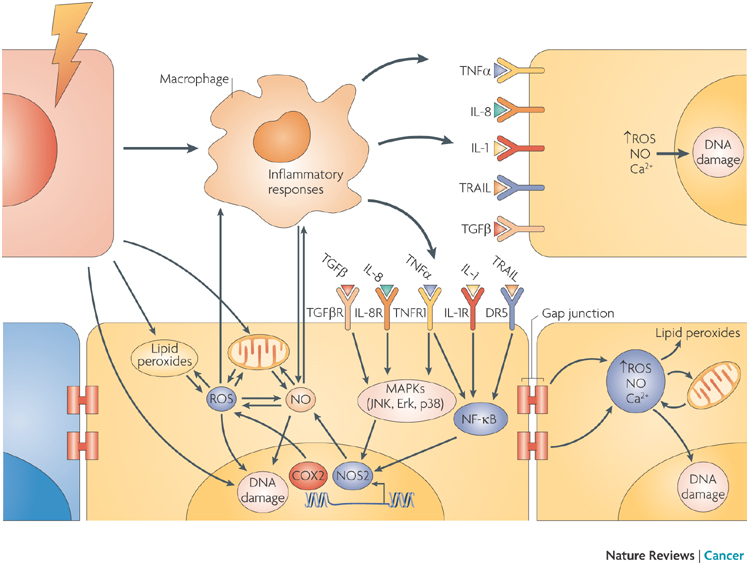
\includegraphics[width=\textwidth]{Key-pathways-affecting-bystander-signals-Cells-respond-to-direct-radiation-red-cell-by}
	
	~\cite{s41416-020-0942-3} Схематический обзор локальных и отдаленных эффектов, вызванных облучением опухоли
	
	
	\subsection{Краткий перечень участвующих в процессах органических соединений, связанных с эндофитами}
	
	\subsubsection{Индолилуксусная кислота}
	Гетероауксин $\beta$-индолилуксусная кислота) — вещество группы ауксинов, производное индола, фитогормон, стимулятор роста растений.
	
	Химическое вещество высокой физиологической активности, образующееся в растениях и влияющее на ростовые процессы (так называемый гормон роста). Один из наиболее широко распространённых ауксинов.
	
	\subsubsection{Гиббереллины}
	Гиббереллины — группа фитогормонов дитерпеновой природы, которые выполняют в растениях разнообразные функции, связанные с контролем удлинения гипокотиля, прорастания семян, зацветания и т. д. В контроле большинства морфогенетических процессов гиббереллины действуют в одном направлении с ауксинами и являются антагонистами цитокининов и абсцизовой кислоты (АБК). ~\cite{GB_1}
	
	\subsubsection{Циркулин}
	
	\subsubsection{Колистин}
		Колистин (Полимиксин E)
	В ноябре 2015 года появились сообщения об обнаружении плазмиды, содержащей ген устойчивости mcr-1 к Полимиксину Е (Colistin)~\cite{Colistin_1}.
	
	\subsubsection{Полимиксин}
	Полимиксины — группа антибиотиков, осуществляющих нарушение цитоплазматической мембраны и обладающих узким спектром активности против грамотрицательной флоры. По химическому составу — это сложные органические соединения, основой которых является полипептид. Естественный продуцент: Bacillus polymyxa и некоторые другие. Основное клиническое значение имеет активность полимиксинов в отношении P. aeruginosa. По химической природе это полиеновые соединения, включающие остатки полипептидов. В обычных дозах препараты этой группы действуют бактериостатически, в высоких концентрациях — оказывают бактерицидное действие.
	
	Из препаратов в основном применяются полимиксин В и полимиксин М. Обладают выраженной нефро- и нейротоксичностью .
	
	
	\subsubsection{Бактериоцины}
Бактериоцины — специфические белки, вырабатываемые некоторыми бактериями и подавляющие жизнедеятельность клеток других штаммов того же вида или родственных видов бактерий. Бактериоцины обозначаются в соответствии с видовым названием, например Escherichia coli образует так называемые колицины (25 типов), Pasteurella pestis — пестицины. Так же Б. подразделяются на типы, в связи с различными признаками, являясь представителями одного вида ~\cite{BC_1}.

Механизм действия бактериоцинов связан с повреждением цитоплазматических мембран белком. Спектр активности бактериоцинов, в отличие от антибиотиков, узок и определяется наличием рецепторов у бактерий для их адсорбции.
	\subsubsection{Экомицин}
	
	\subsubsection{Фенол}
		$C_6H_5OH$
	\subsubsection{Бензол}
	$C_6H_6$
	\subsubsection{Cидерофоры}			
	Cидерофоры (низкомолекулярные вещества, хелатирующие ионы Fe3+) ~\cite{ecogen17119-32}

	\subsection{Краткий перечень участвующих в процессах органических соединений, связанных с радиационно-индуцированной передачей сигналов}
		
	\subsubsection{NF-kB}	
		ядерный фактор kB

	\subsubsection{ROS}	
		Reactive Oxygen species, реактивная форма кислорода

	\subsubsection{RNS}	
		реактивная форма азота

	\subsubsection{COX2}	
		активная форма кислорода, циклооксигеназа-2	

	\subsubsection{NOS2}	
		активная форма азота, NO-синтаза-2	

	\subsubsection{TNFRSF10B}	
		рецептор смерти	

	\subsubsection{IL}	
		интерлейкин

	\subsubsection{JNK}	
		Jun N-терминальная киназа

	\subsubsection{NO}	
		оксид азота

	\subsubsection{$TGF_{\beta}$}	
		трансформирующий фактор роста $\beta$

	\subsubsection{$TGF_{\beta}$R}	
		рецептор $TGF_{\beta}$

	\subsubsection{$TNF_{\alpha}$}	
		фактор некроза опухоли $\alpha$

	\subsubsection{$TRAIL, TNF$}	
		родственный лиганд, индуцирующий апоптоз
		
	\section{Биофизика процесса}
	В ~\cite{nrc2603} приводится иллюстрация возможных последствий при разрушении ДНК:
	
	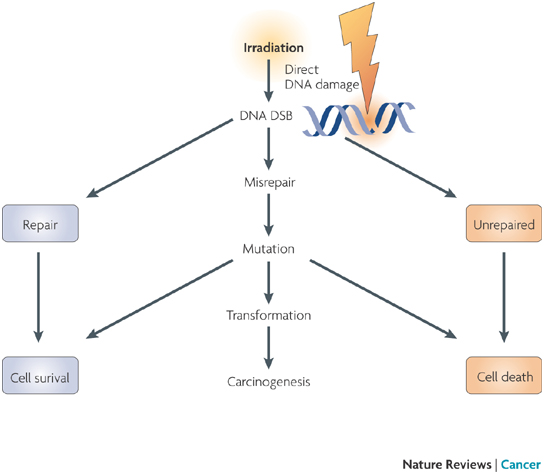
\includegraphics[width=\textwidth]{Direct-DNA-damage-radiation-model-The-schematic-shows-the-standard-model-of-DNA-damage}
	
	\subsection{Ядерные реакции}
	Поскольку мы рассматриваем тепловые нейтроны, то в нашем случае возможен не только процесс ионизации, но и различные, более сложные ядерные реакции на нуклеозидах: рассеяния ~\cite{annurev-biophys-070317-033358} и поглощения ~\cite{Muhin, 27030255}:
	
	\subsubsection{Радиационный захват нейтронов}
	Нейтрон поглощается ядром, а избыток энергии испускается в виде $\gamma$-кванта. Эти реакции характерны для нейтронов с энергиями менее 500 кэВ.
	
	\begin{equation}
	\label{eq1}
	^A_ZX+n \rightarrow ^{A+1}_ZX + \gamma
	\end{equation}

	При этом часто образуется нестабильное ядро, которое претерпевает $\beta$-распад:

	\begin{equation}
	\label{eq2}
	^{A+1}_ZX+ \rightarrow ^{A+1}_{Z+1}X + e^- + \tilde{\nu}
	\end{equation}
	
	\subsubsection{Реакции с образованием протонов}
	Эти реакции наиболее характерны для нейтронов с энергиями 500 кэВ — 10 МэВ.
	
	\begin{equation}
		\label{eq3}
		^A_ZX+n \rightarrow ^A_{Z-1}X + p
	\end{equation}
	
	\subsubsection{Реакции с образованием $\alpha$-частиц}
	Эти реакции также характерны для нейтронов с энергиями 500 кэВ — 10 МэВ, однако в некоторых случаях идут на тепловых нейтронах.
	
	\begin{equation}
		\label{eq4}
		^A_ZX+n \rightarrow ^{A-3}_{Z-2}X + \alpha
	\end{equation}
	
	\subsubsection{Неупругое рассеяние}
	Нейтрон с энергией несколько сот кэВ поглощается ядром, переводит ядро в возбужденное состояние, после чего вылетает из ядра (нельзя сказать, что вылетел тот же самый нейтрон, поскольку нейтроны в ядре неразличимы), но уже с другой энергией.
	
	Сечения каждой реакций $\sigma_{el},\sigma_{un}, \sigma_{n,\gamma}, \sigma_{n,p}, \sigma_{n,\alpha} ... $ приведены в справочнике и могут произойти как в клетке с разным состоянием, так и в структуре во внеклеточном пространстве; испускаемое повторное излучение, после поглощения нейтрона, так же может прореагировать.
	
	\subsection{Биофизическая модель}
	Биофизическая модель может расширятся при добавлении в рассмотрение различных биологических характеристик. На биологическую характеристику влияет множество различных факторов, которые могут быть выбраны в зависимости от сложности модели:
	\begin{itemize} 
	\item состояние клеток
	\item состояние эндофитов
	\item состояние межклеточного пространства
	\item протекающие биохимические реакции
	\item интенсивность и характер облучения
	\item и т.д.
	\end{itemize} 
	
	Нейтроны могут использоваться
	Например, пусть:
			\begin{itemize} 
		\item $v_{grow}$ - скорость роста растения;
		\item $n_{C_{10}H_{9}NO_2}$ - концентрация гетероауксина;
		\item $N$ - интенсивность нейтронного потока;
		\item $v^{burn}_{C_{10}H_{9}NO_2}$ - скорость выгорания гетероауксина;
		\item $v^{prod}_{C_{10}H_{9}NO_2}$ - скорость производства гетероауксина;
		\item $v^{cell}_{C_{10}H_{9}NO_2}$ - скорость производства гетероауксина здоровой клеткой;
		\item $v^{endophyte}_{C_{10}H_{9}NO_2}$ - скорость производства гетероауксина эндофитом;
		\item $k_i$ - коэффициенты пропорциональности;
		\item $c_h$ - количество здоровых клеток;
		\item $c_d$ - количество поврежденных клеток;
		\item $\xi_in$ - приход гетероауксина через ксилемы;
		\item $\xi_in$ - уход гетероауксина через ксилемы;
	\end{itemize} 
	тогда:
		\begin{equation}
		\label{eq5}
		\begin{cases}
			v_{grow} = k_1 n_{C_{10}H_{9}NO_2}/dt \\
			v^{burn}_{C_{10}H_{9}NO_2}= n_{C_{10}H_{9}NO_2}/dt = k_2 N \\
			v^{prod}_{C_{10}H_{9}NO_2} = v^{cell}_{C_{10}H_{9}NO_2} dn_{cell}/dt + v^{endophyte}_{C_{10}H_{9}NO_2} dn_{endophyte}/dt - v^{burn}_{C_{10}H_{9}NO_2} \\
			n_{C_{10}H_{9}NO_2} = k_3 N v^{prod}_{C_{10}H_{9}NO_2}+\xi_in - \xi_out \\
			...
		\end{cases}
	\end{equation}

	и так далее для других параметров. Цель модели - решить задачу оптимизации для подхода MAPs-first.
	
	\section{Информационная модель}
	Информационная модель строится на базе выделенных в результате анализа биохимических и биофизических сущностей и событий, возникающих при обмене сигналами между ними. Диаграмма классов приведена на рисунке:
	
	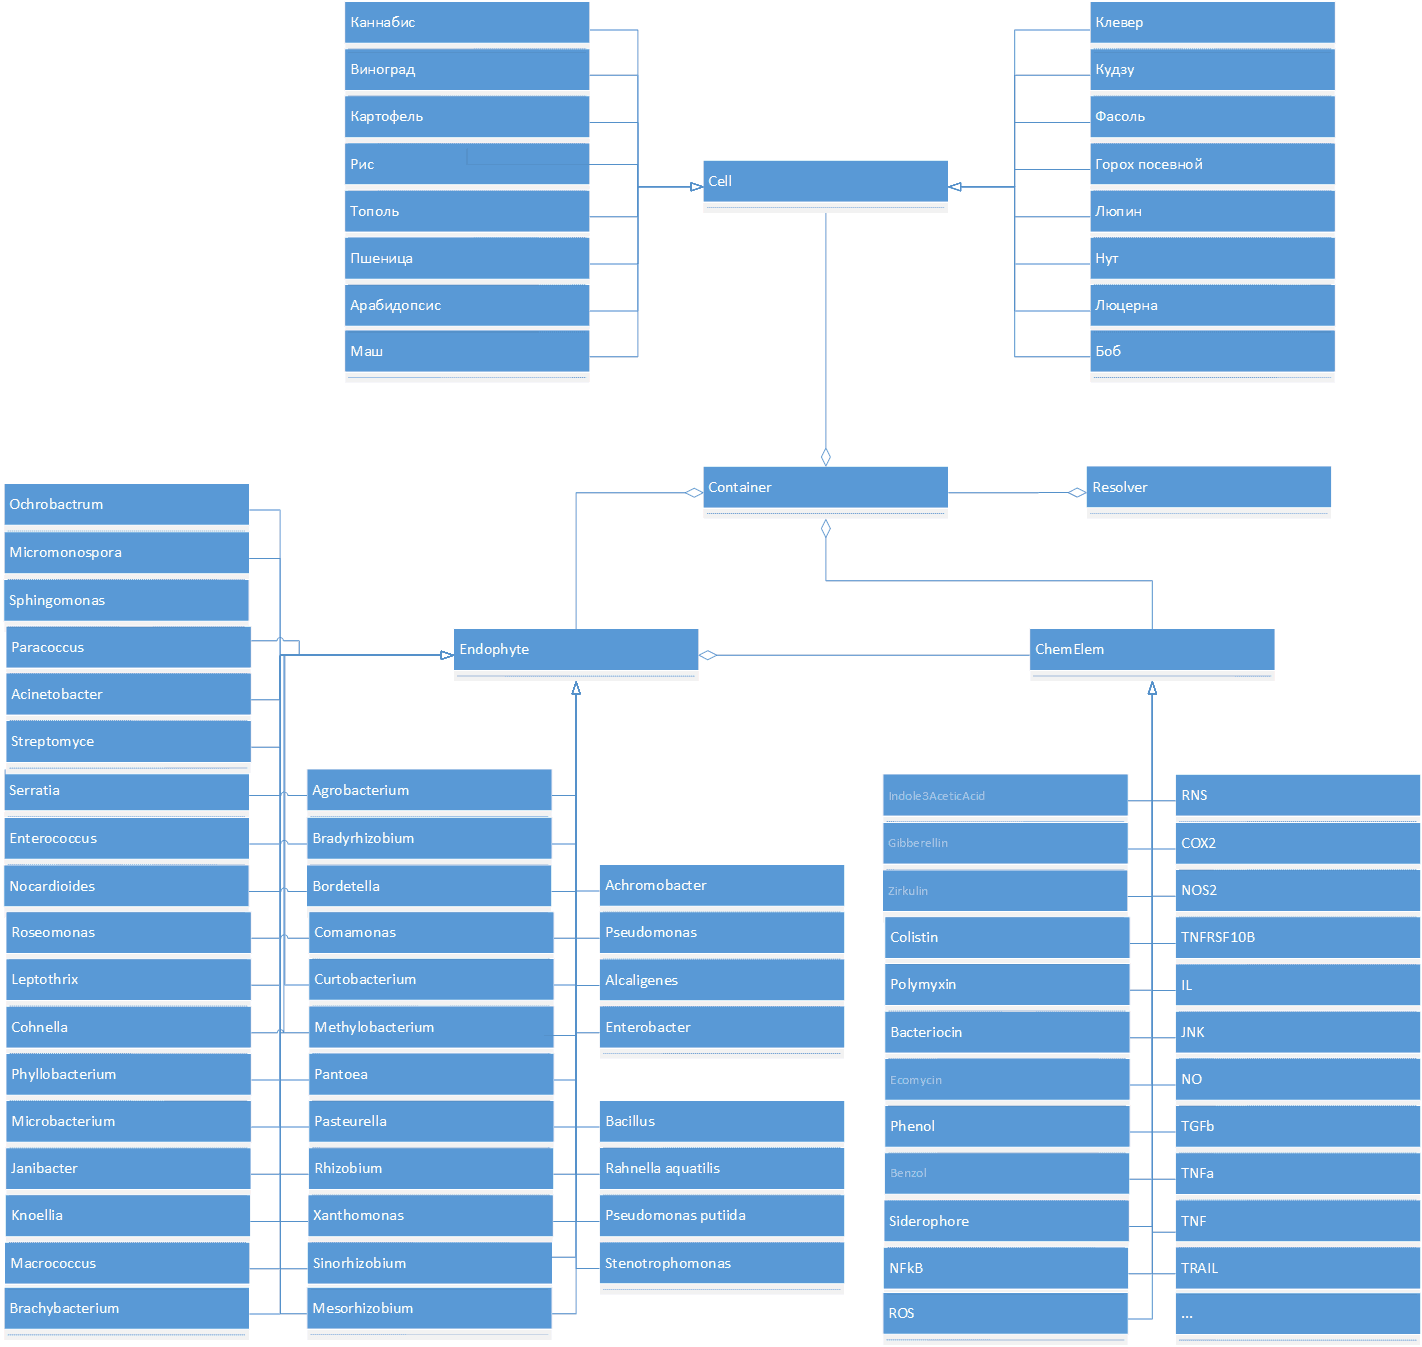
\includegraphics[width=\textwidth]{uml_classes}
	
	Данная модель ~\cite{git} позволит проводить численные эксперименты и результаты сравнивать с экспериментальными данными. Основной практический интерес будет вызывать влияние количественного и качественного наличия эндофитов	в микрофлоре растения.
	
	\section{Заключение}
	Дальнейшее развитие проблематики - концепция «модульного микробиома», представляющего собой микробные консорциумы, разработанные в соответствии с генотипом растения, что придает различные, но взаимодополняющие MAP (MAP — microbiome-associated phenotype;  фенотип, обусловленный микробиомом) отдельному растению-хозяину или целой популяции ~\cite{j.mib.2017.11.023}. Поскольку фактически относительная важность микробиома для роста, развития и здоровья растений не была экспериментально исследована для большинства видов сельскохозяйственных культур, крайне интересным является новый подход MAPs-first, подразумевающий выбор консорциумов и реализующий определенный MAP на основе математических моделей ~\cite{j.mib.2017.11.023}. Полученные данные составят необходимую базу для экспериментов, которая позволит не действовать «вслепую», подбирая стратегии по разработке синтетических эндофитных сообществ ~\cite{ecogen17119-32}.
	Подход MAPs-first можно попробовать перенести и на животный мир, а в перспективе и на человека для снижения отрицательного воздействия внешних факторов, например радиационного воздействия.
	
	\begin{thebibliography}{3}
		\bibitem{ecogen17119-32} Васильева Е.Н., Ахтемова Г.А., Жуков В.А., Тихонович И.А. Эндофитные микроорганизмы в фундаментальных исследованиях и сельском хозяйстве // Экологическая генетика. - 2019. - Т. 17. - №1. - C. 19-32. doi: 10.17816/ecogen17119-32 
		
		\bibitem{09593330.2017.1337232} Iqbal A, Arshad M, Hashmi I, et al. Biodegradation of phenol and benzene by endophytic bacterial strains isolated from refinery wastewater-fed Cannabis sativa. Environ Technol. 2018;39(13):1705-1714. https://doi/org/10.1080/09593330.2017.1337232.
		
		\bibitem{fpls.2011.00100} Partida-Martinez LP, Heil M. The microbe-free plant: fact or artifact? Front Plant Sci. 2011;2:100. https://doi/org/10.3389/fpls.2011.00100.
		
		\bibitem{LRIJ36_4} Narula S, Anand RC, Dudeja SS, Kumar V. Molecular Diversity of Root and Nodule Endophytic Bacteria from Field Pea (Pisum Sativum L.). Legume Res – Int J. 2013;36(4):344-350.
		
		\bibitem{s00248-011-9883-y} Compant S, Mitter B, Colli-Mull JG, et al. Endophytes of grapevine flowers, berries, and seeds: identification of cultivable bacteria, comparison with other plant parts, and visualization of niches of colonization. Microb Ecol. 2011;62(1):188-197. https://doi/org/10.1007/s00248-011-9883-y.
		
		\bibitem{j.tree.2006.11.007} Thrall PH, Hochberg ME, Burdon JJ, Bever JD. Coevo lution of symbiotic mutualists and parasites in a community context. Trends Ecol Evol. 2007;22(3):120-6. https://doi/org/10.1016/j.tree.2006.11.007.
		
		\bibitem{j.micres.2015.11.008} Santoyo G, Moreno-Hagelsieb G, Orozco-Mosqueda Mdel C, Glick BR. Plant growth-promoting bacterial endophytes. Microbiol Res. 2016;183:92-99. https://doi/org/10.1016/j.micres.2015.11.008.
		
		\bibitem{S1286-4579(03)00073-X} Strobel GA. Endophytes as sources of bioactive products. Microbes Infect. 2003;5(6):535-544. https://doi/org/10.1016/S1286-4579(03)00073-X.
		
		\bibitem{b609472b} Zhang HW, Song YC, Tan RX. Biology and chemistry of endophytes. Nat Prod Rep. 2006;23(5):753-771. https://doi/org/10.1039/b609472b.
		
		\bibitem{9781118297674.ch36} Malfanova N, Lugtenberg BJJ, Berg G. Bacterial endophytes: who and where, and what are they doing there? In: Molecular Microbial Ecology of the Rhizosphere. Vol. 1. Ed. by F.J. de Bruijn. Hoboken: John Wiley \& Sons, Ltd.; 2013. https://doi/org/10.1002/9781118297674.ch36.
		
		\bibitem{j.1751-7915.2011.00253.x} Malfanova N, Kamilova F, Validov S, et al. Characterization of Bacillus subtilis HC8, a novel plant-beneficial endophytic strain from giant hogweed. Microb Biotechnol. 2011;4(4):523-532. https://doi/org/10.1111/j.1751-7915.2011.00253.x.
		
		\bibitem{22115501113026660038} Mercado-Blanco J, Lugtenberg B. Biotechnological applications of bacterial endophytes. Curr Biotechnol. 2014;3(1):60-75. https://doi/org/10.2174/22115501113026660038.
		
		\bibitem{j.femsec.2004.08.006} Berg G, Krechel A, Ditz M, et al. Endophytic and ectophytic potato-associated bacterial communities differ in structure and antagonistic function against plant pathogenic fungi. FEMS Microbiol Ecol. 2005;51(2):215-229. https://doi/org/10.1016/j.femsec.2004.08.006.
		
		\bibitem{vol3-issue1-fulltext-4} Azevedo JL, Maccheroni W, Pereira JO, De Araújo WL. Endophytic microorganisms: A review on insect control and recent advances on tropical plants. Electron J Biotechnol. 2000;3(1):40-65. https://doi/org/10.2225/vol3-issue1-fulltext-4.
		
		\bibitem{j.1574-6968.2007.00918.x} Ryan RP, Germaine K, Franks A, et al. Bacterial endophytes: recent developments and applications. FEMS Microbiol Lett. 2008;278(1):1-9. https://doi/org/10.1111/j.1574-6968.2007.00918.x.
		
		\bibitem{S0003683811040090} Maksimov IV, Abizgil’dina RR, Pusenkova LI. Plant growth promoting rhizobacteria as alternative to chemical crop protectors from pathogens (review). Appl Biochem Microbiol. 2011;47(4):333-345. https://doi/org/10.1134/S0003683811040090.
		
		\bibitem{annurev.micro.56.012302.161024} Riley MA, Wertz JE. Bacteriocins: evolution, ecology, and application. Annu Rev Microbiol. 2002;56:117-137. https://doi/org/10.1146/annurev.micro.56.012302.161024.
		
		\bibitem{IPLA_2010_11} Гарипова С.Р., Гарифуллина Д.В., Маркова О.В., и др. Изучение бактериальных ассоциаций эндофитов клубеньков, способствующих увеличению продуктивности бобовых растений // Агрохимия. – 2010. – № 11. – C. 50–58. [Garipova SR, Garifullina DV, Markova OV, et al. Bacterial Endophyte Associations of Nodules Increasing the Productivity of Legumes. Agrokhimiya. 2010;(11):50-58 (In Russ.)]
		
		\bibitem{np030397v} Strobel G, Daisy B, Castillo U, Harper J. Natural products from endophytic microorganisms. J Nat Prod. 2004;67(2):257-268. https://doi/org/10.1021/np030397v.
		
		\bibitem{09593330.2017.1337232} Iqbal A, Arshad M, Hashmi I, et al. Biodegradation of phenol and benzene by endophytic bacterial strains isolated from refinery wastewater-fed Cannabis sativa. Environ Technol. 2018;39(13):1705-1714. https://doi/org/10.1080/09593330.2017.1337232.
		
		\bibitem{s0168-1656(01)00333-9} Verma S. Evaluation of plant growth promoting and colonization ability of endophytic diazotrophs from deep water rice. J Biotechnol. 2001;91(2-3):127-141. https://doi/org/10.1016/s0168-1656(01)00333-9.
		
		\bibitem{MPMI-7-0440} Costa JM, Loper JE. Characterization of siderophore production by the biological control agent enterobacter cloacae. MPMI-Mol Plant Microbe Interact. 1994;7(4):440-448. https://doi/org/10.1094/MPMI-7-0440.
		
		\bibitem{j.0031-9317.2004.00330.x} Pirttila AM, Joensuu P, Pospiech H, et al. Bud endophytes of Scots pine produce adenine derivatives and other compounds that affect morphology and mitigate browning of callus cultures. Physiol Plant. 2004;121(2):305-312. https://doi/org/10.1111/j.0031-9317.2004.00330.x.
		
		\bibitem{AEM.71.9.4951-4959.2005} Compant S, Duffy B, Nowak J, et al. Use of plant growth-promoting bacteria for biocontrol of plant diseases: principles, mechanisms of action, and future prospects. Appl Environ Microbiol. 2005;71(9):4951-9. https://doi/org/10.1128/AEM.71.9.4951-4959.2005.
		
		\bibitem{j.mib.2017.11.023} Oyserman BO, Medema MH, Raaijmakers JM. Road MAPs to engineer host microbiomes. Curr Opin Microbiol. 2018;43:46-54. https://doi/org/10.1016/j.mib.2017.11.023.
		
		\bibitem{nrc2603} Prise, Kevin \& O'Sullivan, Joe. (2009). Radiation-induced bystander signalling in cancer therapy. Nature reviews. Cancer. 9. 351-60. 10.1038/nrc2603. 
		
		\bibitem{27030255} Радиационный захват нейтронов. Справочник - М., ЭНЕРГОАТОМИЗДАТ, 1986
		
		\bibitem{Muhin}  Мухин Экспериментальная ядерная физика - 
		Издательство "Лань", 2008г.
		
		\bibitem{s41416-020-0942-3} Daguenet, E., Louati, S., Wozny, A.-S., Vial, N., Gras, M., Guy, J.-B., … Magné, N. (2020). Radiation-induced bystander and abscopal effects: important lessons from preclinical models. British Journal of Cancer. doi:10.1038/s41416-020-0942-3 
		
		\bibitem{j.apsoil.2015.08.020} Marques JM, da Silva TF, Vollú RE, et al. Bacterial endophytes of sweet potato tuberous roots affected by the plant genotype and growth stage. Appl Soil Ecol. 2015;96:273-281. https://doi/org/10.1016/j.apsoil.2015.08.020.
		
		\bibitem{MPMI-08-11-0204} Sessitsch A, Hardoim P, Doring J, et al. Functional characteristics of an endophyte community colonizing rice roots as revealed by metagenomic analysis. Mol Plant Microbe Interact. 2012;25(1):28-36. https://doi/org/10.1094/MPMI-08-11-0204.
		
		\bibitem{fiv104} Ferrando L, Fernandez Scavino A. Strong shift in the diazotrophic endophytic bacterial community inha biting rice (Oryza sativa) plants after flooding. FEMS Microbiol Ecol. 2015;91(9): fiv104. https://doi/org/10.1093/femsec/fiv104.
		
		\bibitem{s11104-015-2503-8} Ren G, Zhu C, Alam MS, et al. Response of soil, leaf endosphere and phyllosphere bacterial communities to elevated CO2 and soil temperature in a rice paddy. Plant Soil. 2015;392(1-2):27-44. https://doi/org/10.1007/s11104-015-2503-8.
		
		\bibitem{AEM.05255-11} Gottel NR, Castro HF, Kerley M, et al. Distinct microbial communities within the endosphere and rhizosphere of Populus deltoides roots across contrasting soil types. Appl Environ Microbiol. 2011;77(17):5934-44. https://doi/org/10.1128/AEM.05255-11.
		
		\bibitem{fmicb.2017.02552} Liu H, Carvalhais LC, Crawford M, et al. Inner Plant values: diversity, colonization and benefits from endophytic bacteria. Front Microbiol. 2017;8:2552. https://doi/org/10.3389/fmicb.2017.02552.
		
		\bibitem{nature11336} Bulgarelli D, Rott M, Schlaeppi K, et al. Revealing structure and assembly cues for Arabidopsis root-inhabiting bacterial microbiota. Nature. 2012;488(7409):91-95. https://doi/org/10.1038/nature11336.
		
		\bibitem{AJB11.3438} Tariq M, Hameed S, Yasmeen T, Ali A. Non-rhizobial bacteria for improved nodulation and grain yield of mung bean [Vigna radiata (L.) Wilczek]. Afr J Biotechnol 2012;11:15012-15019. https://doi/org/10.5897/AJB11.3438.
		
		\bibitem{17429145.2017.1294212} Egamberdieva D, Wirth S, Jabborova D, et al. Coor dination between Bradyrhizobium and Pseudomonas alleviates salt stress in soybean through altering root system architecture. J Plant In teract. 2017;12(1):100-107. https://doi/org/10.1080/ 17429145.2017.1294212.
		
		\bibitem{s003740050273} Sturz AV, Christie BR, Matheson BG, Nowak J. Biodiversity of endophytic bacteria which colonize red clover nodules, roots, stems and foliage and their influence on host growth. Biol Fertil Soils. 1997;25(1):13-19. https://doi/org/10.1007/s003740050273.
		
		\bibitem{s00284-007-9062-z} Selvakumar G, Kundu S, Gupta AD, et al. Isolation and characterization of nonrhizobial plant growth promoting bacteria from nodules of Kudzu (Pueraria thunbergiana) and their effect on wheat seedling growth. Curr Microbiol. 2008;56(2):134-139. https://doi/org/10.1007/s00284-007-9062-z.
		
		\bibitem{j.syapm.2010.07.005} Lopez-Lopez A, Rogel MA, Ormeno-Orrillo E, et al. Phaseolus vulgaris seed-borne endophytic community with novel bacterial species such as Rhizobium endophyticum sp. nov. Syst Appl Microbiol. 2010;33(6):322-7. https://doi/org/10.1016/j.syapm.2010.07.005.
		
		\bibitem{w00-098} Elvira-Recuenco M, van Vuurde JW. Natural incidence of endophytic bacteria in pea cultivars under field conditions. Can J Microbiol 2000;46(11):1036-1041. https://doi/org/10.1139/w00-098.
			
		\bibitem{ran_2015_1_4} Гарипова С.Р., Гарифуллина Д.В., Маркова О.В., и др. Комплексная биологическая активность in vitro эндофитных бактерий, выделенных из клубеньков гороха и фасоли // Известия Уфимского научного центра Российской академии наук. – 2015. – № 4–1. – С. 25–28. [Garipova SR, Garifullina DV, Markova OV, et al. Complex biological activity in vitro of endophytic bacteria isolated from pea and bean nodules. Izvestiya Ufimskogo Nauchnogo Tsentra Rossiyskoy Akademii Nauk. 2015;(4-1):25-28. (In Russ.)]
		
		\bibitem{j.syapm.2011.11.003} Carro L, Sproer C, Alonso P, Trujillo ME. Diversity of Micromonospora strains isolated from nitrogen fixing nodules and rhizosphere of Pisum sativum analyzed by multilocus sequence analysis. Syst Appl Microbiol. 2012;35(2):73-80. https://doi/org/10.1016/j.syapm.2011.11.003.
			
		\bibitem{j.syapm.2016.04.003} Carro L, Riesco R, Sproer C, Trujillo ME. Micromonospora luteifusca sp. nov. isolated from cultivated Pisum sativum. Syst Appl Microbiol. 2016;39(4):237-42. https://doi/org/10.1016/j.syapm.2016.04.003.
		
		\bibitem{MPMI-18-0169} Iniguez AL, Dong Y, Carter HD, et al. Regulation of enteric endophytic bacterial colonization by plant defenses. Mol Plant Microbe Interact. 2005;18(2):169-78. https://doi/org/10.1094/MPMI-18-0169.
		
		\bibitem{annurev-biophys-070317-033358} Smith, J. C., Tan, P., Petridis, L., \& Hong, L. (2018). Dynamic Neutron Scattering by Biological Systems. Annual Review of Biophysics, 47(1), 335–354. doi:10.1146/annurev-biophys-070317-033358 
		
		\bibitem{j.envres.2019.04.033} Lad, J., Rusin, A., Seymour, C., \& Mothersill, C. (2019). An investigation into neutron-induced bystander effects: How low can you go? Environmental Research, 175, 84–99. doi:10.1016/j.envres.2019.04.033 
		
		\bibitem{09553002.2011.584939} Wang, C., Smith, R. W., Duhig, J., Prestwich, W. V., Byun, S. H., Mcneill, F. E., … Mothersill, C. E. (2011). Neutrons do not produce a bystander effect in zebrafish irradiated in vivo. International Journal of Radiation Biology, 87(9), 964–973. doi:10.3109/09553002.2011.584939
		
		\bibitem{Achromobacter_1} Garrity, George M.; Brenner, Don J.; Krieg, Noel R.; Staley, James T. (eds.) (2005). Bergey's Manual of Systematic Bacteriology, Volume Two: The Proteobacteria, Part C: The Alpha-, Beta-, Delta-, and Epsilonproteobacteria. New York: Springer. ISBN 978-0-387-24145-6.
		
		\bibitem{Achromobacter_2} Gray, JS; Birmingham, JM; Fenton, JI (2010). "Got black swimming dots in your cell culture? Identification of Achromobacter as a novel cell culture contaminant". Biologicals. 38 (2): 273–277. doi:10.1016/j.biologicals.2009.09.006. PMC 2849847. PMID 19926304.
		
		\bibitem{Achromobacter_3} Swenson, Colin E.; Sadikot, Ruxana T. (2015-02-01). "Achromobacter Respiratory Infections". Annals of the American Thoracic Society. 12 (2): 252–258. doi:10.1513/AnnalsATS.201406-288FR. ISSN 2329-6933. PMID 
		
		\bibitem{Alcaligenes_1} "Alcaligenes - Медицинское определение от MediLexicon" . Архивировано из оригинала на 2016-10-09 . Проверено 28 мая 2014 .
		\bibitem{Alcaligenes_2}  Alcaligenes. (n.d.) Miller-Keane Encyclopedia and Dictionary of Medicine, Nursing, and Allied Health, Seventh Edition. (2003). Retrieved May 25 2021 from https://medical-dictionary.thefreedictionary.com/Alcaligenes
		
		\bibitem{Alcaligenes_3} Alcaligenes. (n.d.) Farlex Partner Medical Dictionary. (2012). Retrieved May 25 2021 from https://medical-dictionary.thefreedictionary.com/Alcaligenes
		
		\bibitem{Alcaligenes_4}  Malek-Marín T et al. (2009) A case of endocarditis of difficult diagnosis in dialysis: could "pest" friends be involved? Clin Nephrol 72(5):405-409
		
		\bibitem{Alcaligenes_5} Saiman, L; Chen, Y; Tabibi, S; San Gabriel, P; Zhou, J; Liu, Z; Lai, L; Whittier, S (2001). "Identification and antimicrobial susceptibility of Alcaligenes xylosoxidans isolated from patients with cystic fibrosis". J. Clin. Microbiol. 39 (11): 3942–5. doi:10.1128/JCM.39.11.3942-3945.2001. PMC 88468. PMID 11682511.
		
		\bibitem{Alcaligenes_6} Austin, Brian (2014-01-01). The Family Alcaligenaceae. In Rosenberg, Eugene; DeLong, Edward F.; Lory, Stephen; Stackebrandt, Erko; Thompson, Fabiano (eds.). The Prokaryotes. Springer Berlin Heidelberg. pp. 729–757. doi:10.1007/978-3-642-30197-1\_397. ISBN 9783642301964.
		
		\bibitem{Alcaligenes_7} Kavuncuoglu, F., A. Unal, N. Oguzhan, B. Tokgoz, O. Oymak, and C. Utas. First Reported Case of Alcaligenes Faecalis Peritonitis. Journal of the International Society for Peritoneal Dialysis 30.1 (2010): 118-19. Web. 27 May 2014. <http://www.pdiconnect.com/content/30/1/118.full>
		
		 \bibitem{Enterobacter_1}Adeolu, M.; et al. (2016). "Genome based phylogeny and taxonomy of the 'Enterobacteriales': proposal for Enterobacterales ord. nov. divided into the families Enterobacteriaceae, Erwiniaceae fam. nov., Pectobacteriaceae fam. nov., Yersiniaceae fam. nov., Hafniaceae fam. nov., Morganellaceae fam. nov., and Budviciaceae fam. nov". Int. J. Syst. Evol. Microbiol.
		 
		\bibitem{Enterobacter_2}Tan, Wen-Si; Muhamad Yunos, Nina Yusrina; Tan, Pui-Wan; Mohamad, Nur Izzati; Adrian, Tan-Guan-Sheng; Yin, Wai-Fong; Chan, Kok-Gan (13 June 2014). "Freshwater-Borne Bacteria Isolated from a Malaysian Rainforest Waterfall Exhibiting Quorum Sensing Properties". Sensors. 14 (6): 10527–10537. doi:10.3390/s140610527. PMC 4118381. PMID 24932870.
		
		\bibitem{Enterobacter_3} Cabral, JPS (2010). "Water Microbiology. Bacterial Pathogens and Water". Int. J. Environ. Res. Public Health. 7 (10): 3657–3703. doi:10.3390/ijerph7103657. PMC 2996186. PMID 21139855.
		
		\bibitem{Enterobacter_4} BioMed Central (22 November 2018). "ISS microbes should be monitored to avoid threat to astronaut health". EurekAlert!. Retrieved 25 November 2018.
		
		\bibitem{Enterobacter_5} Singh, Nitin K.; et al. (23 November 2018). "Multi-drug resistant Enterobacter bugandensis species isolated from the International Space Station and comparative genomic analyses with human pathogenic strains". BMC Microbiology. 18 (1): 175. doi:10.1186/s12866-018-1325-2. PMC 6251167. PMID 30466389.
		
		\bibitem{Enterobacter_6} Russo Thomas A, Johnson James R, "Chapter 143. Diseases Caused by Gram-Negative Enteric Bacilli" (Chapter). Fauci AS, Braunwald E, Kasper DL, Hauser SL, Longo DL, Jameson JL, Loscalzo J: Harrison's Principles of Internal Medicine, 17e: http://www.accessmedicine.com/content.aspx?aID=2894446.[dead link]
		
		\bibitem{Enterobacter_7} Wu, Wenjing (19 October 2018). "Enterobacter huaxiensis sp. nov. and Enterobacter chuandaensis sp. nov., recovered from human blood". International Journal of Systematic and Evolutionary Microbiology: 708–714. doi:10.1099/ijsem.0.003207.
		
		\bibitem{Enterobacter_8} Fei, Na; Zhao, Liping (13 December 2012). "An opportunistic pathogen isolated from the gut of an obese human causes obesity in germfree mice". The ISME Journal. 7 (4): 880–4. doi:10.1038/ismej.2012.153. ISSN 1751-7362. PMC 3603399. PMID 23235292.
		
		\bibitem{Acinetobacter_1}  Acinetobacter oryzae ANC 4261 - Project. Genomes OnLine Database (GOLD). Joint Genome Institute (JGI). Retrieved 2021-05-06.
		 
		\bibitem{Acinetobacter_2} Info - Acinetobacter oryzae ANC 4261". Joint Genome Institute Genome Portal. Retrieved 2021-05-06.
		
		\bibitem{Acinetobacter_3} Taxonomy Browser (Acinetobacter oryzae). NCBI Taxonomy Browser. Retrieved 2021-05-06.
		"Species: Acinetobacter oryzae". LPSN (List of Prokaryotic names with Standing in Nomenclature). DSMZ (Deutsche Sammlung von Mikroorganismen und Zellkulturen). Retrieved 2021-05-06.
		
		\bibitem{Acinetobacter_4} Bitrian, Mariana; González, Rodrigo H.; Paris, Gaston; Hellingwerf, Klaas J.; Nudel, Clara B. (2013-09-01). "Blue-light-dependent inhibition of twitching motility in Acinetobacter baylyi ADP1: additive involvement of three BLUF-domain-containing proteins". Microbiology. 159 (Pt 9): 1828–1841. doi:10.1099/mic.0.069153-0. ISSN 1465-2080. PMID 23813679. S2CID 42820743.
		
		\bibitem{Acinetobacter_5} Visca P, Seifert H, Towner KJ (December 2011). "Acinetobacter infection--an emerging threat to human health". IUBMB Life. 63 (12): 1048–54. doi:10.1002/iub.534. PMID 22006724.
		
		\bibitem{Acinetobacter_6} Rokhbakhsh-Zamin, F.; Sachdev, D.P.; Kazemi-Pour, N.; Engineer, A.; Zinjarde, S.S.; Dhakephalkar, P.K.; Chopade, B.A. (2012).
		 Characterization of plant growth promoting traits of Acinetobacter species isolated from rhizosphere of Pennisetum glaucum. J Microbiol Biotechnol. 21 (6): 556–566. doi:10.4014/jmb.1012.12006.
		
		\bibitem{Acinetobacter_7} Antibiotic resistance is a major risk factor for epidemic behavior of Acinetobacter baumannii. Infect Control Hosp Epidemiol 2001; 22:284–288.
		Doughari HJ; Ndakidemi PA; Human IS; Benade S (2011). "The ecology, biology and pathogenesis of Acinetobacter spp.:an overview". Microbes and Environments. 26 (2): 101–112. doi:10.1264/jsme2.me10179. PMID 21502736.
		
		\bibitem{Acinetobacter_8} Dent Lemuel, L; Marshall, DR; Pratap, S; Hulette, RB (2010). "Multidrug resistant Acinetobacter baumannii: a descriptive study in a city hospital". BMC Infect Dis. 10: 196. doi:10.1186/1471-2334-10-196. PMC 2909240. PMID 20609238.
		
		\bibitem{Acinetobacter_9} Siegman-Igra, Y; Bar-Yosef, S; Gorea, A; Avram, J (1993). "Nosocomial Acinetobacter meningitis secondary to invasive procedures: report of 25 cases and review". Clin Infect Dis. 17 (5): 843–849. doi:10.1093/clinids/17.5.843. PMID 8286623.
		
		\bibitem{Acinetobacter_10} Falagas, ME; Karveli, EA; Kelesidis, I; Kelesidis, T (2007). "Community acquired Acinetobacter infections". Eur J Clin Microbiol Infect Dis. 26 (12): 857–868. doi:10.1007/s10096-007-0365-6. PMID 17701432.
		
		\bibitem{Acinetobacter_11} Hu, Q; Hu, Z; Li, J; Tian, B; Xu, H; Li, J (2011). "Detection of OXA-type carbapenemases and integrons among carbapenem-resistant Acinetobactor baumannii in a Teaching Hospital in China". J Basic Microbiol. 51 (5): 467–472. doi:10.1002/jobm.201000402. PMID 21656808.
		
		\bibitem{Acinetobacter_12} Fournier, Pierre Edouard; Richet, H (2006). "The epidemiology and control of Acinetobacter baumannii in healthcare facilities". Clin Infect Dis. 42 (5): 692–699. doi:10.1086/500202. PMID 16447117.
		
	\bibitem{Acinetobacter_13} Peleg AY; Seifert H; Paterson DL (July 2008). "Acinetobacter baumannii: Emergence of a Successful Pathogen". Clinical Microbiology Reviews. 21 (3): 538–582. doi:10.1128/CMR.00058-07. PMC 2493088. PMID 18625687.
		
	\bibitem{Acinetobacter_14} Hanski, I.; Von Hertzen, L.; Fyhrquist, N.; Koskinen, K.; Torppa, K.; Laatikainen, T.; Karisola, P.; Auvinen, P.; Paulin, L.; Makela, M. J.; Vartiainen, E.; Kosunen, T. U.; Alenius, H.; Haahtela, T. (2012). "Environmental biodiversity, human microbiota, and allergy are interrelated". Proceedings of the National Academy of Sciences. 109 (21): 8334–8339. Bibcode:2012PNAS..109.8334H. doi:10.1073/pnas.1205624109. PMC 3361383. PMID 22566627.
		
	\bibitem{Acinetobacter_14} Debarry, J.; Hanuszkiewicz, A.; Stein, K.; Holst, O.; Heine, H. (2009). "The allergy-protective properties of Acinetobacter lwoffii F78 are imparted by its lipopolysaccharide". Allergy. 65 (6): 690–697. doi:10.1111/j.1398-9995.2009.02253.x. PMID 19909295.
		
	\bibitem{Acinetobacter_15} Rahal J (2006). "Novel antibiotic combinations against infections with almost completely resistant Pseudomonas aeruginosa and Acinetobacter species". Clin Infect Dis. 43 Suppl 2: S95–9. doi:10.1086/504486. PMID 16894522.
		
		
	 \bibitem{Bacillus_19} Joan L. Slonczewski \& John W. Foster (2011), Microbiology: An Evolving Science (2nd Edition), Norton

	\bibitem{Bacillus_20} Jeong, Haeyoung; Jeong, Da-Eun; Kim, Sun Hong; Song, Geun Cheol; Park, Soo-Young; Ryu, Choong-Min; Park, Seung-Hwan; Choi, Soo-Keun (2012-08-01). "Draft Genome Sequence of the Plant Growth-Promoting Bacterium Bacillus siamensis KCTC 13613T". Journal of Bacteriology. 194 (15): 4148–4149. doi:10.1128/JB.00805-12. ISSN 0021-9193. PMC 3416560. PMID 22815459.

	\bibitem{Bacillus_21} Keen, E; Bliskovsky, V; Adhya, S; Dantas, G (2017). "Draft genome sequence of the naturally competent Bacillus simplex strain WY10". Genome Announcements. 5 (46): e01295–17. doi:10.1128/genomeA.01295-17. PMC 5690344. PMID 29146837.

	\bibitem{Bacillus_22} Ryan KJ; Ray CG, eds. (2004). Sherris Medical Microbiology (4th ed.). McGraw Hill. ISBN 978-0-8385-8529-0.
		
	\bibitem{Rahnella_aquatilis_1} Asselin JE, Eikemo H, Perminow J, Nordskog B, Brurberg MB, Beer SV. Rahnella spp. are commonly isolated from onion (Allium cepa) bulbs and are weakly pathogenic. J Appl Microbiol. 2019 Sep;127(3):812-824. doi: 10.1111/jam.14340. Epub 2019 Jul 7. PMID: 31161611.
		
	\bibitem{Rahnella_aquatilis_2} Peng J, Wu D, Liang Y, Li L, Guo Y. Disruption of acdS gene reduces plant growth promotion activity and maize saline stress resistance by Rahnella aquatilis HX2. J Basic Microbiol. 2019 Apr;59(4):402-411. doi: 10.1002/jobm.201800510. Epub 2019 Jan 15. PMID: 30644572.
	
	
	\bibitem{Pseudomonas_putiida_1} Anzai; Kim, H; Park, JY; Wakabayashi, H; Oyaizu, H; et al. (Jul 2000). "Phylogenetic affiliation of the pseudomonads based on 16S rRNA sequence". Int J Syst Evol Microbiol. 50 (4): 1563–89. doi:10.1099/00207713-50-4-1563. PMID 10939664.
	 
	\bibitem{Pseudomonas_putiida_2} Nikolaidis, Marios; Mossialos, Dimitris; Oliver, Stephen G.; Amoutzias, Grigorios D. (2020-07-24). "Comparative Analysis of the Core Proteomes among the Pseudomonas Major Evolutionary Groups Reveals Species-Specific Adaptations for Pseudomonas aeruginosa and Pseudomonas chlororaphis". Diversity. 12 (8): 289. doi:10.3390/d12080289. ISSN 1424-2818.
	
	\bibitem{Pseudomonas_putiida_3} Marqués, Silvia; Ramos, Juan L. (1993). "Transcriptional control of the Pseudomonas putida TOL plasmid catabolic pathways". Molecular Microbiology. 9 (5): 923–9. doi:10.1111/j.1365-2958.1993.tb01222.x. PMID 7934920.
	
	\bibitem{Pseudomonas_putiida_4} Gomes, NC; Kosheleva, IA; Abraham, WR; Smalla, K (2005). "Effects of the inoculant strain Pseudomonas putida KT2442 (pNF142) and of naphthalene contamination on the soil bacterial community". FEMS Microbiology Ecology. 54 (1): 21–33. doi:10.1016/j.femsec.2005.02.005. PMID 16329969.
	
	\bibitem{Pseudomonas_putiida_5} Immortal Polystyrene Foam Meets its Enemy | LiveScience

	\bibitem{Pseudomonas_putiida_6} Ward, PG; Goff, M; Donner, M; Kaminsky, W; O'Connor, KE (2006). "A two step chemo-biotechnological conversion of polystyrene to a biodegradable thermoplastic". Environmental Science \& Technology. 40 (7): 2433–7. doi:10.1021/es0517668. PMID 16649270.
	
	\bibitem{Pseudomonas_putiida_7} Amer, GA; Utkhede, RS (2000). "Development of formulations of biological agents for management of root rot of lettuce and cucumber". Canadian Journal of Microbiology. 46 (9): 809–16. doi:10.1139/w00-063. PMID 11006841.
	 
	\bibitem{Pseudomonas_putiida_8} Validov, S; Kamilova, F; Qi, S; Stephan, D; Wang, JJ; Makarova, N; Lugtenberg, B (2007). "Selection of bacteria able to control Fusarium oxysporum f. Sp. Radicis-lycopersici in stonewool substrate". Journal of Applied Microbiology. 102 (2): 461–71. doi:10.1111/j.1365-2672.2006.03083.x. PMID 17241352.
	
	\bibitem{Pseudomonas_putiida9} Cornelis P (editor). (2008). Pseudomonas: Genomics and Molecular Biology (1st ed.). Caister Academic Press. ISBN 1-904455-19-0.
	
	\bibitem{Pseudomonas_putiida_10} ~\url{https://www.researchgate.net/publication/221847539_Industrial_biotechnology_of_Pseudomonas_putida_and_related_species}

	\bibitem{Pseudomonas_putiida_11} ~\url{http://blogs.scientificamerican.com/observations/2011/05/24/newly-discovered-bacteria-lives-on-caffeine}
	
	\bibitem{Pseudomonas_putiida_12} Summers, RM; Louie, TM; Yu, CL; Subramanian, M (2011). "Characterization of a broad-specificity non-haem iron N-demethylase from Pseudomonas putida CBB5 capable of utilizing several purine alkaloids as sole carbon and nitrogen source". Microbiology. 157 (Pt 2): 583–92. doi:10.1099/mic.0.043612-0. PMID 20966097.
	
	\bibitem{Stenotrophomonas_1} ~\url{https://lpsn.dsmz.de/genus/stenotrophomonas}
	
	\bibitem{Stenotrophomonas_2} Palleroni N, Bradbury J (1993). "Stenotrophomonas, a new bacterial genus for Xanthomonas maltophilia (Hugh 1980) Swings et al. 1983". Int J Syst Bacteriol. 43 (3): 606–9. doi:10.1099/00207713-43-3-606. PMID 8347518.
	
	\bibitem{Stenotrophomonas_3} Ryan, Robert P.; Monchy, Sebastien; Cardinale, Massimiliano; Taghavi, Safiyh; Crossman, Lisa; Avison, Matthew B.; Berg, Gabriele; van der Lelie, Daniel; Dow, J. Maxwell (2009). "The versatility and adaptation of bacteria from the genus Stenotrophomonas". Nature Reviews Microbiology. 7 (7): 514–525. doi:10.1038/nrmicro2163. ISSN 1740-1526. PMID 19528958.
	
	\bibitem{Stenotrophomonas_4} Hauben L, Vauterin L, Moore E, Hoste B, Swings J (1999). "Genomic diversity of the genus Stenotrophomonas". Int J Syst Bacteriol. 49 (4): 1749–60. doi:10.1099/00207713-49-4-1749. PMID 10555357.
	
	\bibitem{Stenotrophomonas_5} Aykac, Kubra; Ozsurekci, Yasemin; Tuncer, Ozlem; Sancak, Banu; Cengiz, Ali Bulent; Kara, Ates; Ceyhan, Mehmet (2016). "Six cases during 2012–2015 and literature review of Chryseobacterium indologenes infections in pediatric patients". Canadian Journal of Microbiology. 62 (10): 812–819. doi:10.1139/cjm-2015-0800. ISSN 0008-4166. PMID 27397741.
	
	\bibitem{Stenotrophomonas_6} Coenye, Tom; Vanlaere, Elke; LiPuma, John J; Vandamme, Peter (2004). "Identification of genomic groups in the genus Stenotrophomonas using gyrB RFLP analysis". FEMS Immunology \& Medical Microbiology. 40 (3): 181–185. doi:10.1016/S0928-8244(03)00307-9. PMID 15039092.
	
	\bibitem{Stenotrophomonas_7} Svensson-Stadler, Liselott A.; Mihaylova, Sashka A.; Moore, Edward R.B. (2012). "Stenotrophomonas interspecies differentiation and identification by gyrB sequence analysis". FEMS Microbiology Letters. 327 (1): 15–24. doi:10.1111/j.1574-6968.2011.02452.x. PMID 22092789.
	
	\bibitem{Stenotrophomonas_8} Rocco, Francesco; De Gregorio, Eliana; Di Nocera, Pier Paolo (2010). "A giant family of short palindromic sequences in Stenotrophomonas maltophilia: Stenotrophomonas maltophilia REPs". FEMS Microbiology Letters: no. doi:10.1111/j.1574-6968.2010.02010.x
	
	
	\bibitem{Agrobacterium_1} Uchino Y, Yokota A, Sugiyama J (August 1997). "Phylogenetic position of the marine subdivision of Agrobacterium species based on 16S rRNA sequence analysis". The Journal of General and Applied Microbiology. 43 (4): 243–247. doi:10.2323/jgam.43.243. PMID 12501326.
	
	\bibitem{Agrobacterium_2} Uchino Y, Hirata A, Yokota A, Sugiyama J (June 1998). "Reclassification of marine Agrobacterium species: Proposals of Stappia stellulata gen. nov., comb. nov., Stappia aggregata sp. nov., nom. rev., Ruegeria atlantica gen. nov., comb. nov., Ruegeria gelatinovora comb. nov., Ruegeria algicola comb. nov., and Ahrensia kieliense gen. nov., sp. nov., nom. rev". The Journal of General and Applied Microbiology. 44 (3): 201–210. doi:10.2323/jgam.44.201. PMID 12501429.
	
	\bibitem{Agrobacterium_3} Young JM, Kuykendall LD, Martínez-Romero E, Kerr A, Sawada H (January 2001). "A revision of Rhizobium Frank 1889, with an emended description of the genus, and the inclusion of all species of Agrobacterium Conn 1942 and Allorhizobium undicola de Lajudie et al. 1998 as new combinations: Rhizobium radiobacter, R. rhizogenes, R. rubi, R. undicola and R. vitis". International Journal of Systematic and Evolutionary Microbiology. 51 (Pt 1): 89–103. doi:10.1099/00207713-51-1-89. PMID 11211278.[permanent dead link]
	
	\bibitem{Agrobacterium_4} Farrand SK, van Berkum PB, Oger P (September 2003). "Agrobacterium is a definable genus of the family Rhizobiaceae". International Journal of Systematic and Evolutionary Microbiology. 53 (Pt 5): 1681–1687. doi:10.1099/ijs.0.02445-0. PMID 13130068.
	
	\bibitem{Agrobacterium_5} Young JM, Kuykendall LD, Martínez-Romero E, Kerr A, Sawada H (September 2003). "Classification and nomenclature of Agrobacterium and Rhizobium". International Journal of Systematic and Evolutionary Microbiology. 53 (Pt 5): 1689–1695. doi:10.1099/ijs.0.02762-0. PMID 13130069.
	
	\bibitem{Agrobacterium_6} Sawada H, Ieki H, Oyaizu H, Matsumoto S (October 1993). "Proposal for rejection of Agrobacterium tumefaciens and revised descriptions for the genus Agrobacterium and for Agrobacterium radiobacter and Agrobacterium rhizogenes". International Journal of Systematic Bacteriology. 43 (4): 694–702. doi:10.1099/00207713-43-4-694. PMID 8240952.
	
	\bibitem{Agrobacterium_7} Francis KE, Spiker S (February 2005). "Identification of Arabidopsis thaliana transformants without selection reveals a high occurrence of silenced T-DNA integrations". The Plant Journal. 41 (3): 464–77. doi:10.1111/j.1365-313X.2004.02312.x. PMID 15659104.
	
	\bibitem{Agrobacterium_8} Pitzschke A, Hirt H (March 2010). "New insights into an old story: Agrobacterium-induced tumour formation in plants by plant transformation". The EMBO Journal. 29 (6): 1021–32. doi:10.1038/emboj.2010.8. PMC 2845280. PMID 20150897.
	
	\bibitem{Agrobacterium_9} Hulse M, Johnson S, Ferrieri P (January 1993). "Agrobacterium infections in humans: experience at one hospital and review". Clinical Infectious Diseases. 16 (1): 112–7. doi:10.1093/clinids/16.1.112. PMID 8448285.
	
	\bibitem{Agrobacterium_10} Dunne WM, Tillman J, Murray JC (September 1993). "Recovery of a strain of Agrobacterium radiobacter with a mucoid phenotype from an immunocompromised child with bacteremia". Journal of Clinical Microbiology. 31 (9): 2541–3. doi:10.1128/JCM.31.9.2541-2543.1993. PMC 265809. PMID 8408587.
	
	\bibitem{Agrobacterium_11} Cain JR (March 1988). "A case of septicaemia caused by Agrobacterium radiobacter". The Journal of Infection. 16 (2): 205–6. doi:10.1016/s0163-4453(88)94272-7. PMID 3351321.
	
	\bibitem{Agrobacterium_12} Kunik T, Tzfira T, Kapulnik Y, Gafni Y, Dingwall C, Citovsky V (February 2001). "Genetic transformation of HeLa cells by Agrobacterium". Proceedings of the National Academy of Sciences of the United States of America. 98 (4): 1871–6. Bibcode:2001PNAS...98.1871K. doi:10.1073/pnas.041327598. JSTOR 3054968. PMC 29349. PMID 11172043.
	
	\bibitem{Agrobacterium_13} Schell J, Van Montagu M (1977). "The Ti-Plasmid of Agrobacterium tumefaciens, A Natural Vector for the Introduction of NIF Genes in Plants?". In Hollaender A, Burris RH, Day PR, Hardy RW, Helinski DR, Lamborg MR, Owens L, Valentine RC (eds.). Genetic Engineering for Nitrogen Fixation. Basic Life Sciences. 9. pp. 159–79. doi:10.1007/978-1-4684-0880-5\_12. ISBN 978-1-4684-0882-9. PMID 336023.
	
	\bibitem{Agrobacterium_14} Joos H, Timmerman B, Montagu MV, Schell J (1983). "Genetic analysis of transfer and stabilization of Agrobacterium DNA in plant cells". The EMBO Journal. 2 (12): 2151–60. doi:10.1002/j.1460-2075.1983.tb01716.x. PMC 555427. PMID 16453483.
	
	\bibitem{Agrobacterium_15} Thomson JA. "Genetic Engineering of Plants" (PDF). Biotechnology. 3. Archived (PDF) from the original on 17 January 2017. Retrieved 17 July 2016.
	
	\bibitem{Agrobacterium_16} Leuzinger K, Dent M, Hurtado J, Stahnke J, Lai H, Zhou X, Chen Q (July 2013). "Efficient agroinfiltration of plants for high-level transient expression of recombinant proteins". Journal of Visualized Experiments. 77 (77). doi:10.3791/50521. PMC 3846102. PMID 23913006.
	
	\bibitem{Agrobacterium_17} Shamloul M, Trusa J, Mett V, Yusibov V (April 2014). "Optimization and utilization of Agrobacterium-mediated transient protein production in Nicotiana". Journal of Visualized Experiments (86). doi:10.3791/51204. PMC 4174718. PMID 24796351.
	
	\bibitem{Agrobacterium_18} Clough SJ, Bent AF (December 1998). "Floral dip: a simplified method for Agrobacterium-mediated transformation of Arabidopsis thaliana". The Plant Journal. 16 (6): 735–43. doi:10.1046/j.1365-313x.1998.00343.x. PMID 10069079.
	
	\bibitem{Agrobacterium_19} The FDA List of Completed Consultations on Bioengineered Foods Archived May 13, 2008, at the Wayback Machine
	\bibitem{Agrobacterium_20} Michielse CB, Hooykaas PJ, van den Hondel CA, Ram AF (July 2005). "Agrobacterium-mediated transformation as a tool for functional genomics in fungi". Current Genetics. 48 (1): 1–17. doi:10.1007/s00294-005-0578-0. PMID 15889258. S2CID 23959400.
	
	\bibitem{Agrobacterium_21} Idnurm A, Bailey AM, Cairns TC, Elliott CE, Foster GD, Ianiri G, Jeon J (2017). "Agrobacterium-mediated transformation of fungi". Fungal Biology and Biotechnology. 4: 6. doi:10.1186/s40694-017-0035-0. PMC 5615635. PMID 28955474.
	
	\bibitem{Agrobacterium_22}Setubal JC, Wood D, Burr T, Farrand SK, Goldman BS, Goodner B, Otten L, Slater S (2009). "The Genomics of Agrobacterium: Insights into its Pathogenicity, Biocontrol, and Evolution". In Jackson RW (ed.). Plant Pathogenic Bacteria: Genomics and Molecular Biology. Caister Academic Press. pp. 91–112. ISBN 978-1-904455-37-0.
	
	\bibitem{Bradyrhizobium_1}
	 Ramirez-Bahena, M.-H.; Chahboune, R.; Peix, A.; Velazquez, E. (2012). "Reclassification of Agromonas oligotrophica into the genus Bradyrhizobium as Bradyrhizobium oligotrophicum comb. nov". International Journal of Systematic and Evolutionary Microbiology. 63 (Pt 3): 1013–6. doi:10.1099/ijs.0.041897-0. PMID 22685107.
	 
	\bibitem{Bradyrhizobium_2} Eaglesham AR, Ellis JM, Evans WR, Fleishman DE, Hungria M, Hardy KW (1990). "The first photosynthetic N2-fixing Rhizobium: Characteristics". In Gresshoff PM, Koth LE, Stacey G, Newton WE (eds.). Nitrogen Fixation: Achievements and Objectives. Boston, MA: Springer. pp. 805–811. doi:10.1007/978-1-4684-6432-0\_69. ISBN 978-1-4684-6434-4.
	
	\bibitem{Bradyrhizobium_3} VanInsberghe, David; Maas, Kendra; Cardenas, Erick; Strachan, Cameron; Hallam, Steven; Mohn, William (2015). "Non-symbiotic Bradyrhizobium ecotypes dominate North American forest soils". The ISME Journal. 9 (11): 2435–2441. doi:10.1038/ismej.2015.54. PMC 4611507. PMID 25909973.
	
	\bibitem{Bradyrhizobium_4} P. Somasegaran (1994). Handbook for rhizobia: Methods in legume–rhizobium technology. New York: Springer-Verlag. pp. 1–6, 167. ISBN 978-0-387-94134-9.
	
	\bibitem{Bradyrhizobium_5} Gary, King (2003). "Molecular and culture-based analyses of aerobic carbon monoxide oxidizer diversity". Applied and Environmental Microbiology. 69 (12): 7257–7265. doi:10.1128/aem.69.12.7257-7265.2003. PMC 309980. PMID 14660374.
	
	\bibitem{Bradyrhizobium_6} "List of Prokaryotic names with Standing in Nomenclature —Bradyrhizobium". Retrieved May 23, 2021.
	
	\bibitem{Bradyrhizobium_7} Klepa MS, Ferraz Helene LC, O'Hara G, Hungria M. (2021). "Bradyrhizobium agreste sp. nov., Bradyrhizobium glycinis sp. nov. and Bradyrhizobium diversitatis sp. nov., isolated from a biodiversity hotspot of the genus Glycine in Western Australia". Int J Syst Evol Microbiol. doi:10.1099/ijsem.0.004742. PMID 33709900.
	
	\bibitem{Bradyrhizobium_8} Kalita, M; Małek, W (2010). "Genista tinctoria microsymbionts from Poland are new members of Bradyrhizobium japonicum bv. genistearum". Systematic and Applied Microbiology. 33 (5): 252–9. doi:10.1016/j.syapm.2010.03.005. PMID 20452160.
	
	\bibitem{Bradyrhizobium_9} Stacey, Gary (1995). "Bradyrhizobium japonicum nodulation genetics". FEMS Microbiology Letters. 127 (1–2): 1–9. doi:10.1111/j.1574-6968.1995.tb07441.x. PMID 7737469.
	
	\bibitem{Bradyrhizobium_10} Stacey, G; Sanjuan, J.; Luka, S.; Dockendorff, T.; Carlson, R.W. (1995). "Signal exchange in the Bradyrhizobium–soybean symbiosis". Soil Biology and Biochemistry. 27 (4–5): 473–483. doi:10.1016/0038-0717(95)98622-U.
	
	\bibitem{Bradyrhizobium_11} Caetanoanolles, G (1997). "Molecular dissection and improvement of the nodule symbiosis in legumes". Field Crops Research. 53 (1–3): 47–68. doi:10.1016/S0378-4290(97)00022-1.
	
	\bibitem{Bradyrhizobium_12} van Berkum, P.; Sloger, C.; Weber, D. F.; Cregan, P. B.; Keyser, H. H. (1985). "Relationship between Ureide N and N2 Fixation, Aboveground N Accumulation, Acetylene Reduction, and Nodule Mass in Greenhouse and Field Studies with Glycine max (L.) Merr". Plant Physiol. 77 (1): 53–58. doi:10.1104/pp.77.1.53. PMC 1064455. PMID 16664027.
	
	\bibitem{Bradyrhizobium_13} Hennecke, H (1990). "Nitrogen fixation genes involved in the Bradyrhizobium japonicum–soybean symbiosis". FEBS Letters. 268 (2): 422–6. doi:10.1016/0014-5793(90)81297-2. PMID 2200721.
	
	\bibitem{Bradyrhizobium_14} Rivas, Raul; Martens, Miet; De Lajudie, Philippe; Willems, Anne (2009). "Multilocus sequence analysis of the genus Bradyrhizobium". Systematic and Applied Microbiology. 32 (2): 101–10. doi:10.1016/j.syapm.2008.12.005. PMID 19201125.
	
	\bibitem{Bradyrhizobium_15} Chaintreuil, Clémence; Giraud, Eric; Prin, Yves; Lorquin, Jean; Bâ, Amadou; Gillis, Monique; de Lajudie, Philippe; Dreyfus, Bernard (December 2000). "Photosynthetic Bradyrhizobia Are Natural Endophytes of the African Wild Rice Oryza breviligulata". Applied and Environmental Microbiology. 66 (12): 5437–5447. doi:10.1128/AEM.66.12.5437-5447.2000. Retrieved 7 May 2021.
	
	\bibitem{Bradyrhizobium_16}Alberton, O; Kaschuk, G; Hungria, M (2006). "Sampling effects on the assessment of genetic diversity of rhizobia associated with soybean and common bean". Soil Biology and Biochemistry. 38 (6): 1298–1307. doi:10.1016/j.soilbio.2005.08.018.
	
	\bibitem{Bradyrhizobium_17}Salter, S; Cox, M; Turek, E; Calus, S; Cookson, W; Moffatt, M; Turner, P; Parkhill, J; Loman, N; Walker, A (2014). "Reagent contamination can critically impact sequence-based microbiome analyses". bioRxiv 10.1101/007187.
	
	\bibitem{Bradyrhizobium_18} Kulakov, L; McAlister, M; Ogden, K; Larkin, M; O'Hanlon, J (2002). "Analysis of Bacteria Contaminating Ultrapure Water in Industrial Systems". Applied and Environmental Microbiology. 68 (4): 1548–1555. doi:10.1128/AEM.68.4.1548-1555.2002. PMC 123900. PMID 11916667.
		
	\bibitem{Bordetella_1}
	~\url{https://www.ncbi.nlm.nih.gov/Taxonomy/Browser/wwwtax.cgi?mode=Tree\&id=517\&lvl=3\&keep=1\&srchmode=1\&unlock}
		
	\bibitem{Bordetella_2} Ryan KJ; Ray CG, eds. (2004). Sherris Medical Microbiology (4th ed.). McGraw Hill. ISBN 978-0-8385-8529-0.
	
	\bibitem{Bordetella_3} Hewlett, Erik L.; Damron, F. Heath; Wong, Ting; Fernandez, Julieta; Sisti, Federico; Zacca, Federico; Gonyar, Laura A.; Hoffman, Casandra L. (2019-06-25). «Bordetella pertussis Can Be Motile and Express Flagellum-Like Structures». mBio (en inglés) 10(3): e00787-19. ISSN 2150-7511. PMID 31088927 |pmid=incorrecto (ayuda). doi:10.1128/mBio.00787-19

	\bibitem{Bordetella_4} Bauwens J, Spach D, Schacker T, Mustafa M, Bowden R (1992). "Bordetella bronchiseptica pneumonia and bacteremia following bone marrow transplantation". J Clin Microbiol. 30 (9): 2474–5. PMC 265527. PMID 1401019.
	
	\bibitem{Bordetella_5} Hewlett E (1997). "Pertussis: current concepts of pathogenesis and prevention". Pediatr Infect Dis J. 16 (4 Suppl): S78–84. doi:10.1097/00006454-199704001-00002. PMID 9109161.
	
	\bibitem{Bordetella_6} Cotter PA, Miller JF (2001). Groisman EA (ed.). Bordetella. Principles of Bacterial Pathogenesis. Academic Press. pp. 619–674. doi:10.1016/B978-012304220-0/50014-5. ISBN 978-0-12-304220-0.
	
	\bibitem{Bordetella_7} Mattoo S, Cherry J (2005). "Molecular Pathogenesis, Epidemiology, and Clinical Manifestations of Respiratory Infections Due to Bordetella pertussis and Other Bordetella Subspecies". Clin Microbiol Rev. 18 (2): 326–82. doi:10.1128/CMR.18.2.326-382.2005. PMC 1082800. PMID 15831828.
	
	\bibitem{Bordetella_8} Gray MC, Donato GM, Jones FR, Kim T, Hewlett EL (2004). "Newly secreted adenylate cyclase toxin is responsible for intoxication of target cells by Bordetella pertussis". Mol. Microbiol. 53 (6): 1709–19. doi:10.1111/j.1365-2958.2004.04227.x. PMID 15341649.
	
	\bibitem{Bordetella_9} Hewlett EL, Donato GM, Gray MC (2006). "Macrophage cytotoxicity produced by adenylate cyclase toxin from Bordetella pertussis: more than just making cyclic AMP!". Mol. Microbiol. 59 (2): 447–59. doi:10.1111/j.1365-2958.2005.04958.x. PMID 16390441.
	
	\bibitem{Bordetella_10} Fiser R, Masín J, Basler M, Krusek J, Spuláková V, Konopásek I, Sebo P (2007). "Third activity of Bordetella adenylate cyclase (AC) toxin-hemolysin. Membrane translocation of AC domain polypeptide promotes calcium influx into CD11b+ monocytes independently of the catalytic and hemolytic activities". J. Biol. Chem. 282 (5): 2808–20. doi:10.1074/jbc.M609979200. PMID 17148436.
	
	\bibitem{Bordetella_11}Uhl M, Miller J (1994). "Autophosphorylation and phosphotransfer in the Bordetella pertussis BvgAS signal transduction cascade". Proc Natl Acad Sci USA. 91 (3): 1163–7. Bibcode:1994PNAS...91.1163U. doi:10.1073/pnas.91.3.1163. PMC 521474. PMID 8302847.
	
	\bibitem{Bordetella_12} Steffen P, Goyard S, Ullmann A (1996). "Phosphorylated BvgA is sufficient for transcriptional activation of virulence-regulated genes in Bordetella pertussis". EMBO J. 15 (1): 102–9. doi:10.1002/j.1460-2075.1996.tb00338.x. PMC 449922. PMID 8598192.
	
	\bibitem{Bordetella_13} Akerley B, Monack D, Falkow S, Miller J (1992). "The bvgAS locus negatively controls motility and synthesis of flagella in Bordetella bronchiseptica". J Bacteriol. 174 (3): 980–90. doi:10.1128/jb.174.3.980-990.1992. PMC 206178. PMID 1370665.
	
	\bibitem{Bordetella_14} Merkel T, Stibitz S (1995). "Identification of a locus required for the regulation of bvg-repressed genes in Bordetella pertussis". J Bacteriol. 177 (10): 2727–36. doi:10.1128/jb.177.10.2727-2736.1995. PMC 176943. PMID 7751282.
	
	\bibitem{Bordetella_15}Beattie D, Mahan M, Mekalanos J (1993). "Repressor binding to a regulatory site in the DNA coding sequence is sufficient to confer transcriptional regulation of the vir-repressed genes (vrg genes) in Bordetella pertussis". J Bacteriol. 175 (2): 519–27. doi:10.1128/jb.175.2.519-527.1993. PMC 196167. PMID 8419298.
	
	\bibitem{Bordetella_16} Cotter P, Miller J (1997). "A mutation in the Bordetella bronchiseptica bvgS gene results in reduced virulence and increased resistance to starvation, and identifies a new class of Bvg-regulated antigens". Mol Microbiol. 24 (4): 671–85. doi:10.1046/j.1365-2958.1997.3821741.x. PMID 9194696.
	
	\bibitem{Bordetella_17} van den Akker W (1997). "Bordetella bronchiseptica has a BvgAS-controlled cytotoxic effect upon interaction with epithelial cells". FEMS Microbiol Lett. 156 (2): 239–44. doi:10.1016/S0378-1097(97)00431-X. PMID 9513272.
	
	\bibitem{Bordetella_18} "How Frequently Does A Dog Need A Bordetella Vaccine?". Cornerstone Animal Hospital. Retrieved 22 October 2020.
	
	\bibitem{Comamonas_1} ~\url{https://lpsn.dsmz.de/genus/comamonas}
	
	~\bibitem{Comamonas_2} Garrity, George M.; Brenner, Don J.; Krieg, Noel R.; Staley, James T. (eds.) (2005). Bergey's Manual of Systematic Bacteriology, Volume Two: The Proteobacteria, Part C: The Alpha-, Beta-, Delta-, and Epsilonproteobacteria. New York, New York: Springer. ISBN 978-0-387-24145-6.
	 
	~\bibitem{Curtobacterium_1} Guido Funke; Max Aravena-Roman; Reinhard Frodl (22 November 2004). "First Description of Curtobacterium spp. Isolated from Human Clinical Specimens". Journal of Clinical Microbiology. 43 (3): 1032–1036. doi:10.1128/JCM.43.3.1032-1036.2005. PMC 1081300. PMID 15750056.
	
	~\bibitem{Curtobacterium_2} Alexander B Chase; Philip Arevalo; Martin F Polz; Renaud Berlemont; Jennifer B H Martiny (November 22, 2016). "Evidence for Ecological Flexibility in the Cosmopolitan Genus Curtobacterium". Frontiers in Microbiology. 7 (1874): 1874. doi:10.3389/fmicb.2016.01874. PMC 5118839. PMID 27920771.
	
	~\bibitem{Methylobacterium_1}
	~\url{https://lpsn.dsmz.de/genus/methylobacterium}
	
	~\bibitem{Methylobacterium_2} Garrity, George M.; Brenner, Don J.; Krieg, Noel R.; Staley, James T. (eds.) (2005). Bergey's Manual of Systematic Bacteriology, Volume Two: The Proteobacteria, Part C: The Alpha-, Beta-, Delta-, and Epsilonproteobacteria. New York, New York: Springer. ISBN 978-0-387-24145-6.
	
	~\bibitem{Methylobacterium_3} Salter, S; Cox, M; Turek, E; Calus, S; Cookson, W; Moffatt, M; Turner, P; Parkhill, J; Loman, N; Walker, A (2014). "Reagent contamination can critically impact sequence-based microbiome analyses". bioRxiv 10.1101/007187.
	
	~\bibitem{Methylobacterium_4} Bowler, Jacinta (16 March 2021). "Microbes Unknown to Science Discovered on The International Space Station". ScienceAlert. Retrieved 16 March 2021.
	
	~\bibitem{Methylobacterium_5} Rogers, Adam (April 5, 2021). "Sneaky New Bacteria on the ISS Could Build a Future on Mars". Wired. One species, found on a HEPA filter in the station’s life-support system, was a garden-variety (literally!) Methylobacterium rhodesianum. But three samples—from a surface near the materials research rack, a wall near the “cupola” of windows, and the astronauts' dining table—were something new.
	
	~\bibitem{Methylobacterium_6} O'Connor M, Wopat A, Hanson RS (1977). "Genetic transformation in Methylobacterium organophilum". J. Gen. Microbiol. 98 (1): 265–72. doi:10.1099/00221287-98-1-265. PMID 401866.
	
	~\bibitem{Methylobacterium_7} Euzéby JP, Parte AC. "Methylobacteriaceae". List of Prokaryotic names with Standing in Nomenclature (LPSN). Retrieved May 22, 2021.
	
	~\bibitem{Methylobacterium_8} Bijlani S, Singh NK, Eedara VVR, Podile AR, Mason CE, Wang CCC, Venkateswaran K. (2021). "Methylobacterium ajmalii sp. nov., Isolated From the International Space Station". Front Microbiol. 12: 639396. doi:10.3389/fmicb.2021.639396.
	
	~\bibitem{Pantoea_1} Walterson, Alyssa M.; Stavrinides, John (2015-11-01). "Pantoea: insights into a highly versatile and diverse genus within the Enterobacteriaceae". FEMS Microbiology Reviews. 39 (6): 968–984. doi:10.1093/femsre/fuv027. ISSN 1574-6976. PMID 26109597.
	
	~\bibitem{Pantoea_2} Donnenberg, Michael (2009). Mandell, Douglas, and Bennett's Principles and Practice of Infectious Diseases. Chapter 218: Enterobacteriaceae. p. 2827.

	~\bibitem{Pantoea_3} Tan, Wen-Si; Muhamad Yunos, Nina Yusrina; Tan, Pui-Wan; Mohamad, Nur Izzati; Adrian, Tan-Guan-Sheng; Yin, Wai-Fong; Chan, Kok-Gan (12 August 2014). "Pantoea sp. Isolated from Tropical Fresh Water Exhibiting N-Acyl Homoserine Lactone Production". The Scientific World Journal. 2014 (2014): 828971. doi:10.1155/2014/828971. PMC 4146356. PMID 25197715.
	
	~\bibitem{Pantoea_4} Delétoile, Alexis; Decré, Dominique; Courant, Stéphanie; Passet, Virginie; Audo, Jennifer; Grimont, Patrick; Arlet, Guillaume; Brisse, Sylvain (2009-02-01). "Phylogeny and Identification of Pantoea Species and Typing of Pantoea agglomerans Strains by Multilocus Gene Sequencing". Journal of Clinical Microbiology. 47 (2): 300–310. doi:10.1128/JCM.01916-08. ISSN 0095-1137. PMC 2643697. PMID 19052179.
	
	~\bibitem{Pantoea_5} Donnenberg, Michael (2015). "Enterobacteriaceae". Mandell, Douglas, and Bennett's Principles and Practice of Infectious Diseases, 8th Edition. pp. 2503–2517.e5. ISBN 978-1-4557-4801-3.

	~\bibitem{Pantoea_6} GAVINI, F.; MERGAERT, J.; BEJI, A.; MIELCAREK, C.; IZARD, D.; KERSTERS, K.; LEY, J. DE (1989-07-01). "Transfer of Enterobacter agglomerans (Beijerinck 1888) Ewing and Fife 1972 to Pantoea gen. nov. as Pantoea agglomerans comb. nov. and Description of Pantoea dispersa sp. nov". International Journal of Systematic Bacteriology. 39 (3): 337–345. doi:10.1099/00207713-39-3-337.
	
	~\bibitem{Pasteurella_1} "Pasteurella". List of Prokaryotic Names with Standing in Nomenclature. Retrieved 2006-04-06.
	
	~\bibitem{Pasteurella_2} Kuhnert P; Christensen H, eds. (2008). Pasteurellaceae: Biology, Genomics and Molecular Aspects. Caister Academic Press. ISBN 978-1-904455-34-9.
	
	~\bibitem{Pasteurella_3} Health Protection Agency (2007). Identification of Pasteurella species and morphologically similar bacteria (.pdf) Archived 2009-09-22 at the Wayback Machine. National Standard Method BSOP ID 13 Issue 2.1.

	~\bibitem{Pasteurella_4} "Pasteurella". Introduction To Clinical Microbiology. Archived from the original on 2006-01-16. Retrieved 2006-04-06.
	
	~\bibitem{Pasteurella_5} Mark A Marinella, MD. "Community-Acquired Pneumonia Due to Pasteurella multocida" (PDF). Archived from the original (PDF) on 2016-03-03. Retrieved 2007-09-15.
	
	~\bibitem{Pasteurella_6} Collins, Frank M. (1996-01-01). Baron, Samuel (ed.). Pasteurella, Yersinia, and Francisella (4th ed.). Galveston (TX): University of Texas Medical Branch at Galveston. ISBN 0963117211. PMID 21413268.
	
	~\bibitem{Pasteurella_7} Collins FM (1996). Barron S; et al. (eds.). Pasteurella, Yersinia, and Francisella. In: Baron's Medical Microbiology (4th ed.). Univ of Texas Medical Branch. ISBN 0-9631172-1-1. (via NCBI Bookshelf).

	~\bibitem{Pasteurella_8} "In vitro Antimicrobial Susceptibility of Pasteurella Mutocida" (PDF). Pakistan Journal of Agriculture, Agriculture Engineering and Veterinary Sciences.
	
	~\bibitem{Pasteurella_9} Ahmad, Ahmad TA; Rammah; Sheweita; Haroun; El-Sayed (2014). "Development of immunization trials against Pasteurella multocida". Vaccine. 32 (8): 909–917. doi:10.1016/j.vaccine.2013.11.068.
	
	~\bibitem{Pasteurella_10} Ahmad, Ahmad TA; Rammah; Sheweita; Haroun; El-Sayed (2018). "The enhancement of the Pasteurella's bacterin by propolis extracts". Reports of Biochemistry and Molecular Biology. 6 (2): 208–218. PMC 5941127. PMID 29766005.
	
	~\bibitem{Pasteurella_11} El-Ashry ESH, Ahmad TA; Ahmad TA. "The use of propolis as vaccine's adjuvant". Vaccine. 31: 1. doi:10.1016/j.vaccine.2012.10.095.
	
	~\bibitem{Pasteurella_12} Barbara Deeb, DVM, MS Assistant Professor Dept. of Comparative Medicine University of Washington. "Pasteurella multocida Infection in Rabbits".

	~\bibitem{Pasteurella_13} "Human Rabies Prevention, United States, Recommendations of the Advisory Committee on Immunization Practices" (PDF). Centers for Disease Control and Prevention, Morbidity and Mortality Weekly Report. 2008. p. 2. Retrieved April 25, 2017.  This article incorporates public domain material from websites or documents of the Centers for Disease Control and Prevention.

	~\bibitem{Pasteurella_14} Okoh, A.E.J. (1980). An outbreak of pasteurellosis in Kano Zoo. Journal of Wildlife Diseases 16: 3–5.
	
	~\bibitem{Pasteurella_15} Wells, M.Y. and Montali, R.J. (1985). Pasteurellosis in southern potoroos. Journal of Zoo Animal Medicine 16: 21–25.
	
	~\bibitem{Pasteurella_16} "Pets and Pasteurella Infections". healthy children.org. June 27, 2012. Retrieved July 18, 2012.
	
	~\bibitem{Rhizobium_1}  Euzéby JP. "Rhizobium". List of Prokaryotic names with Standing in Nomenclature (LPSN). Retrieved 2012-05-02.
	
	~\bibitem{Rhizobium_2} Sawada H, Kuykendall LD, Young JM (June 2003). "Changing concepts in the systematics of bacterial nitrogen-fixing legume symbionts". The Journal of General and Applied Microbiology. 49 (3): 155–79. doi:10.2323/jgam.49.155. PMID 12949698.
	
	~\bibitem{Rhizobium_3} Sridevi M, Mallaiah KV (March 2009). "Phosphate solubilization by Rhizobium strains". Indian Journal of Microbiology. 49 (1): 98–102. doi:10.1007/s12088-009-0005-1. PMC 3450048. PMID 23100757.
	
	~\bibitem{Rhizobium_4} Young JM, Kuykendall LD, Martínez-Romero E, Kerr A, Sawada H (January 2001). "A revision of Rhizobium Frank 1889, with an emended description of the genus, and the inclusion of all species of Agrobacterium Conn 1942 and Allorhizobium undicola de Lajudie et al. 1998 as new combinations: Rhizobium radiobacter, R. rhizogenes, R. rubi, R. undicola and R. vitis". International Journal of Systematic and Evolutionary Microbiology. 51 (Pt 1): 89–103. doi:10.1099/00207713-51-1-89. PMID 11211278.
	
	~\bibitem{Rhizobium_5} "Marvelous Microbe Collections Accelerate Discoveries To Protect People, Plants—and More!". Agricultural Research. United States Department of Agriculture. January 2010. Retrieved 10 August 2018.
	
	~\bibitem{Rhizobium_6} Salter SJ, Cox MJ, Turek EM, Calus ST, Cookson WO, Moffatt MF, et al. (November 2014). "Reagent and laboratory contamination can critically impact sequence-based microbiome analyses". BMC Biology. 12: 87. bioRxiv 10.1101/007187. doi:10.1186/s12915-014-0087-z. PMC 4228153. PMID 25387460.
	
	~\bibitem{Rhizobium_7} Kulakov LA, McAlister MB, Ogden KL, Larkin MJ, O'Hanlon JF (April 2002). "Analysis of bacteria contaminating ultrapure water in industrial systems". Applied and Environmental Microbiology. 68 (4): 1548–55. doi:10.1128/AEM.68.4.1548-1555.2002. PMC 123900. PMID 11916667.
	
	~\bibitem{Rhizobium_8} Amarger N, Macheret V, Laguerre G (October 1997). "Rhizobium gallicum sp. nov. and Rhizobium giardinii sp. nov., from Phaseolus vulgaris nodules". International Journal of Systematic Bacteriology. 47 (4): 996–1006. doi:10.1099/00207713-47-4-996. PMID 9336898.
	
	~\bibitem{Rhizobium_9}Silva C, Vinuesa P, Eguiarte LE, Souza V, Martínez-Romero E (November 2005). "Evolutionary genetics and biogeographic structure of Rhizobium gallicum sensu lato, a widely distributed bacterial symbiont of diverse legumes". Molecular Ecology. 14 (13): 4033–50. doi:10.1111/j.1365-294X.2005.02721.x. PMID 16262857. S2CID 16668742.
	
	~\bibitem{Rhizobium_10} Diange EA, Lee SS (June 2013). "Rhizobium halotolerans sp. nov., Isolated from chloroethylenes contaminated soil". Current Microbiology. 66 (6): 599–605. doi:10.1007/s00284-013-0313-x. PMID 23377488. S2CID 17809044.
	
	~\bibitem{Rhizobium_11} Marek-Kozaczuk M, Leszcz A, Wielbo J, Wdowiak-Wróbel S, Skorupska A (June 2013). "Rhizobium pisi sv. trifolii K3.22 harboring nod genes of the Rhizobium leguminosarum sv. trifolii cluster". Systematic and Applied Microbiology. 36 (4): 252–8. doi:10.1016/j.syapm.2013.01.005. PMID 23507586.
	
	~\bibitem{Rhizobium_12} Kesari V, Ramesh AM, Rangan L (2013). "Rhizobium pongamiae sp. nov. from root nodules of Pongamia pinnata". BioMed Research International. 2013: 165198. doi:10.1155/2013/165198. PMC 3783817. PMID 24078904.
	
	~\bibitem{Rhizobium_13} Xu L, Zhang Y, Deng ZS, Zhao L, Wei XL, Wei GH (March 2013). "Rhizobium qilianshanense sp. nov., a novel species isolated from root nodule of Oxytropis ochrocephala Bunge in China". Antonie van Leeuwenhoek. 103 (3): 559–65. doi:10.1007/s10482-012-9840-x. PMID 23142858. S2CID 18660422.
	
	~\bibitem{Rhizobium_14} Turdahon M, Osman G, Hamdun M, Yusuf K, Abdurehim Z, Abaydulla G, et al. (July 2013). "Rhizobium tarimense sp. nov., isolated from soil in the ancient Khiyik River". International Journal of Systematic and Evolutionary Microbiology. 63 (Pt 7): 2424–2429. doi:10.1099/ijs.0.042176-0. PMID 23203621. S2CID 19459097.
	
	~\bibitem{Rhizobium_15} Wang F, Wang ET, Wu LJ, Sui XH, Li Y, Chen WX (November 2011). "Rhizobium vallis sp. nov., isolated from nodules of three leguminous species". International Journal of Systematic and Evolutionary Microbiology. 61 (Pt 11): 2582–2588. doi:10.1099/ijs.0.026484-0. PMID 21131504.
	
	~\bibitem{Rhizobium_16} Sayers; et al. "Rhizobium/Agrobacterium group". National Center for Biotechnology Information (NCBI) taxonomy database. Retrieved 2012-05-02.
	
	~\bibitem{Rhizobium_17} All-Species Living Tree Project."16S rRNA-based LTP release 106 (full tree)" (PDF). Silva Comprehensive Ribosomal RNA Database. Retrieved 2012-05-02.

	~\bibitem{Rhizobium_18} Arthrobacter viscosus is currently classified in the Micrococcaceae. See Arthrobacter.
	
	~\bibitem{Xanthomonas_1} An SQ, Potnis N, Dow M, Vorhölter FJ, He YQ, Becker A, et al. (October 2019). "Mechanistic insights into host adaptation, virulence and epidemiology of the phytopathogen Xanthomonas". FEMS Microbiology Reviews. 44 (1): 1–32. doi:10.1093/femsre/fuz024. PMID 31578554.
	
	~\bibitem{Xanthomonas_2} Doidge EM (1921). "A tomato canker". Annals of Applied Biology. 7 (4): 407–30. doi:10.1111/j.1744-7348.1921.tb05528.x.
	
	~\bibitem{Xanthomonas_3} Dowson WJ (1939). "On the systematic position and generic names of the Gram-negative bacterial plant pathogens". Zentralblatt für Bakteriologie, Parasitenkunde, Infektionskrankheiten und Hygiene.: 177–193.
	
	~\bibitem{Xanthomonas_4} Young JM, Dye DW, Bradbury JF, Panagopoulos CG, Robbs CF (1978). "A proposed nomenclature and classification for plant pathogenic bacteria". New Zealand Journal of Agricultural Research. 21 (1): 153–177. doi:10.1080/00288233.1978.10427397. ISSN 0028-8233.
	
	~\bibitem{Xanthomonas_5}Stall RE, Beaulieu C, Egel DS (1994). "Two genetically diverse groups of strains are included in Xanthomonas campestris pv. vesicatoria". Int J Syst Bacteriol. 44: 47–53. doi:10.1099/00207713-44-1-47.
	
	~\bibitem{Xanthomonas_6} Vauterin L, Swings J, Kersters K, Gillis M, Mew TW, Schroth MN, et al. (1990). "Towards an improved taxonomy of Xanthomonas". Int J Syst Bacteriol. 40 (3): 312–316. doi:10.1099/00207713-40-3-312.
	
	~\bibitem{Xanthomonas_7} Rademaker JL, Louws FJ, Schultz MH, Rossbach U, Vauterin L, Swings J, de Bruijn FJ (September 2005). "A comprehensive species to strain taxonomic framework for xanthomonas". Phytopathology. 95 (9): 1098–111. doi:10.1094/phyto-95-1098. PMID 18943308.
	
	~\bibitem{Xanthomonas_8} Vauterin L, Hoste B, Kersters K, Swings J (1995). "Reclassification of Xanthomonas". Int J Syst Evol Microbiol. 45 (3): 472–489. doi:10.1099/00207713-45-3-472.
	
	~\bibitem{Xanthomonas_9} Ah-You N, Gagnevin L, Grimont PA, Brisse S, Nesme X, Chiroleu F, et al. (February 2009). "Polyphasic characterization of xanthomonads pathogenic to members of the Anacardiaceae and their relatedness to species of Xanthomonas". International Journal of Systematic and Evolutionary Microbiology. 59 (Pt 2): 306–18. doi:10.1099/ijs.0.65453-0. PMID 19196770.
	
	~\bibitem{Xanthomonas_10} Young JM, Wilkie JP, Park DS, Watson DR (2010). "New Zealand strains of plant pathogenic bacteria classified by multi-locus sequence analysis; proposal of Xanthomonas dyei sp. nov". Plant Pathol. 59 (2): 270–281. doi:10.1111/j.1365-3059.2009.02210.x.
	
	~\bibitem{Xanthomonas_11} Rodriguez-R LM, Grajales A, Arrieta-Ortiz ML, Salazar C, Restrepo S, Bernal A (March 2012). "Genomes-based phylogeny of the genus Xanthomonas". BMC Microbiology. 12: 43. doi:10.1186/1471-2180-12-43. PMC 3359215. PMID 22443110.
	
	~\bibitem{Xanthomonas_12} Büttner D, Bonas U (March 2010). "Regulation and secretion of Xanthomonas virulence factors". FEMS Microbiology Reviews. 34 (2): 107–33. doi:10.1111/j.1574-6976.2009.00192.x. PMID 19925633.
	
	~\bibitem{Xanthomonas_13} Studholme, David J.; Wicker, Emmanuel; Abrare, Sadik Muzemil; Aspin, Andrew; Bogdanove, Adam; Broders, Kirk; Dubrow, Zoe; Grant, Murray; Jones, Jeffrey B.; Karamura, Georgina; Lang, Jillian; Leach, Jan; Mahuku, George; Nakato, Gloria Valentine; Coutinho, Teresa; Smith, Julian; Bull, Carolee T. (2020). "Transfer of Xanthomonas campestris pv. arecae and X. campestris pv. musacearum to X. vasicola (Vauterin) as X. vasicola pv. arecae comb. nov. and X. vasicola pv. musacearum comb. nov. and Description of X. vasicola pv. vasculorum pv. nov". Phytopathology. American Phytopathological Society. 110 (6): 1153–1160. doi:10.1094/phyto-03-19-0098-le. ISSN 0031-949X.
	
	~\bibitem{Xanthomonas_14} Schaad NW, Jones JB, Chun W (2001). "Laboratory Guide for Identification of Plant Pathogenic Bacteria 3rd Ed": 175–199.
	
	~\bibitem{Xanthomonas_15} Boch J, Bonas U (September 2010). "Xanthomonas AvrBs3 family-type III effectors: discovery and function". Annual Review of Phytopathology. 48: 419–36. doi:10.1146/annurev-phyto-080508-081936. PMID 19400638.
	
	~\bibitem{Xanthomonas_16} Ritchie DF (2000). "Bacterial spot of pepper and tomato". The Plant Health Instructor. doi:10.1094/PHI-I-2000-1027-01.
	
	~\bibitem{Xanthomonas_17} Mew TW, Alvarez AM, Leach JE, Swings J (1993). "Focus on bacterial blight of rice". Plant Disease. 77: 5–13. doi:10.1094/pd-77-0005.
	
	~\bibitem{Xanthomonas_18}Hajri A, Brin C, Hunault G, Lardeux F, Lemaire C, Manceau C, et al. (August 2009). Yang CH (ed.). "A "repertoire for repertoire" hypothesis: repertoires of type three effectors are candidate determinants of host specificity in Xanthomonas". PLOS ONE. 4 (8): e6632. Bibcode:2009PLoSO...4.6632H. doi:10.1371/journal.pone.0006632. PMC 2722093. PMID 19680562.
	
	~\bibitem{Xanthomonas_19} Souza DP, Oka GU, Alvarez-Martinez CE, Bisson-Filho AW, Dunger G, Hobeika L, et al. (March 2015). "Bacterial killing via a type IV secretion system". Nature Communications. 6 (1): 6453. Bibcode:2015NatCo...6.6453S. doi:10.1038/ncomms7453. PMID 25743609.
	
	~\bibitem{Xanthomonas_20} Bayer-Santos E, Lima LD, Ceseti LM, Ratagami CY, de Santana ES, da Silva AM, et al. (April 2018). "Xanthomonas citri T6SS mediates resistance to Dictyostelium predation and is regulated by an ECF $\sigma$ factor and cognate Ser/Thr kinase". Environmental Microbiology. 20 (4): 1562–1575. doi:10.1111/1462-2920.14085. PMID 29488354. S2CID 3579518.
	
	~\bibitem{Xanthomonas_21} Ellis SD, Boehm MJ, Coplin D (2008). "Bacterial Diseases of Plants". Ohio State University Fact Sheet.
	~\bibitem{Xanthomonas_22} Koebnik R (7 August 2012), The Xanthomonas Resource
	
	~\bibitem{Sinorhizobium_21}  Galibert F, Finan TM, Long SR, Puhler A, Abola P, Ampe F, et al. (July 2001). "The composite genome of the legume symbiont Sinorhizobium meliloti". Science. 293 (5530): 668–72. doi:10.1126/science.1060966. PMID 11474104.
	
	~\bibitem{Sinorhizobium_22} "NCBI Genome Page for Sinorhizobium meliloti". National Center for Biotechnology Information (NCBI).

	~\bibitem{Sinorhizobium_23}"NCBI Genome Page for Sinorhizobium medicae". National Center for Biotechnology Information (NCBI).
	
	~\bibitem{Sinorhizobium_24}Schmeisser C, Liesegang H, Krysciak D, Bakkou N, Le Quéré A, Wollherr A, Heinemeyer I, Morgenstern B, Pommerening-Röser A, Flores M, Palacios R, Brenner S, Gottschalk G, Schmitz RA, Broughton WJ, Perret X, Strittmatter AW, Streit WR (June 2009). "Rhizobium sp. strain NGR234 possesses a remarkable number of secretion systems". Applied and Environmental Microbiology. 75 (12): 4035–45. doi:10.1128/AEM.00515-09. PMC 2698369. PMID 19376903.
	
	~\bibitem{Sinorhizobium_25} "NCBI Genome Page for Sinorhizobium fredii". National Center for Biotechnology Information (NCBI).
	Young JM (November 2003)
	
	~\bibitem{Mesorhizobium_1}Kaneko, T.; et al. (2000). "Complete Genome Structure of the Nitrogen-fixing Symbiotic Bacterium Mesorhizobium loti". DNA Research. 7 (6): 331–338. doi:10.1093/dnares/7.6.331. PMID 11214968.
	
	~\bibitem{Mesorhizobium_2}"List of Prokaryotic names with Standing in Nomenclature—Mesorhizobium". Retrieved May 25, 2021.
	
	~\bibitem{Mesorhizobium_3}Parte, A.C. "Mesorhizobium". LPSN.
	
	~\bibitem{Mesorhizobium_4}De Meyer SE, Andrews M, James EK, Willems A. (2019). "Mesorhizobium carmichaelinearum sp. nov., isolated from Carmichaelineae spp. root nodules". Int J Syst Evol Microbiol. 69 (1): 146–152. doi:10.1099/ijsem.0.003120. PMID 30457516.
	
	~\bibitem{Mesorhizobium_5} Lo, S. C.; Li, B.; Hung, G. C.; Lei, H.; Li, T.; Zhang, J.; Nagamine, K.; Tsai, S.; Zucker, M. J.; Olesnicky, L. (2013). "Isolation and Characterization of Two Novel Bacteria Afipia cberi and Mesorhizobium hominis from Blood of a Patient Afflicted with Fatal Pulmonary Illness". PLoS ONE. 8 (12): e82673. Bibcode:2013PLoSO...882673L. doi:10.1371/journal.pone.0082673. PMC 3867388. PMID 24367538.
	
	
	~\bibitem{Serratia_5} Khanna, Ashish; Khanna, Menka; Aggarwal, Aruna (February 2013). "Serratia Marcescens- A Rare Opportunistic Nosocomial Pathogen and Measures to Limit its Spread in Hospitalized Patients". Journal of Clinical and Diagnostic Research. 7 (2): 243–246. doi:10.7860/JCDR/2013/5010.2737. ISSN 2249-782X. PMC 3592283. PMID 23543704.
	
	~\bibitem{Serratia_21} Haddix, Pryce L.; Shanks, Robert M. Q. (September 2018). "Prodigiosin pigment of Serratia marcescens is associated with increased biomass production". Archives of Microbiology. 200 (7): 989–999. doi:10.1007/s00203-018-1508-0. ISSN 1432-072X. PMC 7815229. PMID 29616306. S2CID 4566478.
	
	~\bibitem{Serratia_22}Clements, T.; Ndlovu, T.; Khan, S.; Khan, W. (19 November 2018). "Biosurfactants produced by Serratia species: Classification, biosynthesis, production and application". Applied Microbiology and Biotechnology. 103 (2): 589–602. doi:10.1007/s00253-018-9520-5. ISSN 0175-7598. PMID 30456577. S2CID 53874159.
	
	~\bibitem{Serratia_23} Araújo, Hélvia W. C.; Andrade, Rosileide F. S.; Montero-Rodríguez, Dayana; Rubio-Ribeaux, Daylin; Alves da Silva, Carlos A.; Campos-Takaki, Galba M. (4 January 2019). "Sustainable biosurfactant produced by Serratia marcescens UCP 1549 and its suitability for agricultural and marine bioremediation applications". Microbial Cell Factories. 18 (1): 2. doi:10.1186/s12934-018-1046-0. ISSN 1475-2859. PMC 6318876. PMID 30609918.
	
	~\bibitem{Serratia_24} Benedik, M. J., \& Strych, U. (1998). Serratia marcescens and its extracellular nuclease. FEMS Microbiology Letters, 165(1), 1–13. doi: 10.1111/j.1574-6968.1998.tb13120.x
	
	~\bibitem{Serratia_25} Garcia-Silvera, Edgar Edurman, 
	Martinez-Morales, Fernando; Bertrand, Brandt;Morales-Guzman, Daniel; Rosas-Galvan, Nashbly Sarela; Leon-Rodriguez, Renato; Trejo-Hernandez, Maria R. (2018). "Production and application of a thermostable lipase from Serratia marcescens in detergent formulation and biodiesel production". Biotechnology and Applied Biochemistry. 65 (2): 156–172. doi:10.1002/bab.1565. ISSN 1470-8744. PMID 28444972. S2CID 4920172.
	
	~\bibitem{Serratia_26} Pinna, Antonio; Usai, Donatella; Sechi, Leonardo A.; Carta, Arturo; Zanetti, Stefania (2011). "Detection of virulence factors in Serratia strains isolated from contact lens-associated corneal ulcers". Acta Ophthalmologica. 89 (4): 382–387. doi:10.1111/j.1755-3768.2009.01689.x. ISSN 1755-3768. PMID 19845561. S2CID 1979103.
	
	~\bibitem{Serratia_27} Ruan, Yuan; Braum, Volkmar (1 August 1990). "Hemolysin as a marker for Serratia". Archives of Microbiology. 154 (3): 221–225. doi:10.1007/BF00248958. ISSN 1432-072X. PMID 2222120. S2CID 12924027.
	
	~\bibitem{Serratia_28} Joshi, Sadhna; Kozlowski, Maya (1987), "Cloning of Serratia Liquefaciens Chitinase Gene(s)", Molecular genetics of plant-microbe interactions, Springer Netherlands, pp. 328–330, doi:10.1007/978-94-009-4482-4\_83, ISBN 978-94-010-8496-3
	
	~\bibitem{Serratia_29} Fuchs, R. L.; McPherson, S. A.; Drahos, D. J. (1987), "Cloning and Expression of a Serratia Marcescens Gene Encoding Chitinase", Plant Pathogenic Bacteria, Springer Netherlands, p. 478, doi:10.1007/978-94-009-3555-6\_101, ISBN 978-94-010-8090-3
	
	~\bibitem{Serratia_30} Preobrazhenskaya, Yu. V.; Voskoboev, A. I.; Burd, V. N. (1 November 2003). "Hydrolysis of Phosphoester Bond by the Heme-Independent Chloroperoxidase from Serratia marcescens". Russian Journal of Bioorganic Chemistry. 29 (6): 556–559. doi:10.1023/B:RUBI.0000008896.40862.d6. ISSN 1573-9163. S2CID 12145365.
	
	~\bibitem{Serratia_31} Preiss, J; Crawford, K; Downey, J; Lammel, C; Greenberg, E (July 1976). "Kinetic properties of Serratia marcescens adenosine 5'-diphosphate glucose pyrophosphorylase". Journal of Bacteriology. 127 (1): 193–203. doi:10.1128/JB.127.1.193-203.1976. ISSN 0021-9193. PMC 233051. PMID 6432.
	
	~\bibitem{Enterococcus_1} ~\url{https://lpsn.dsmz.de/genus/enterococcus}
	
	~\bibitem{Enterococcus_4} Gilmore MS; et al., eds. (2002). The Enterococci: Pathogenesis, Molecular Biology, and Antibiotic Resistance. Washington, D.C.: ASM Press. ISBN 978-1-55581-234-8.
	
	~\bibitem{Nocardioides_1} ~\url{https://lpsn.dsmz.de/genus/nocardioides}
	
	~\bibitem{Nocardioides_4}  Yoon, Jung-Hoon; Park, Yong-Ha (1 January 2006). "The Genus Nocardioides". The Prokaryotes. Springer New York: 1099–1113. doi:10.1007/0-387-30743-5\_44.
	
	~\bibitem{Nocardioides_5} ~\url{https://www.uniprot.org/taxonomy/1839}

	~\bibitem{Roseomonas_1}
	Qiu X, Qu Z, Jiang F, Lin Y, Zhang Y, Chang X, Da X, Deng S, Kim M, Fang C, Peng F. Roseomonas arctica sp. nov., isolated from arctic glacial foreland soil. International Journal of Systematic and Evolutionary Microbiology. 2016 Mar 1;66(3):1218-23.
	
	~\bibitem{Roseomonas_2}
	Kim DU, Lee H, Kim SG, Ka JO. Roseomonas terricola sp. nov., isolated from agricultural soil. International Journal of Systematic and Evolutionary Microbiology. 2017 Oct 6.

	~\bibitem{Leptothrix_1} Parte, Aidan C.; Euzéby, Jean P. "Genus Leptothrix". List of Prokaryotic names with Standing in Nomenclature. Retrieved 15 December 2017.
	
	~\bibitem{Leptothrix_2} "Leptothrix". NCBI taxonomy. Bethesda, MD: National Center for Biotechnology Information. Retrieved 14 December 2017. Other names: synonym: Detoniella Trevisan in de Toni and Trevisan 1889 synonym: Chlamydothrix synonym: "Chlamydothrix" Migula 1900 Lineage( full ) cellular organisms; Bacteria; Proteobacteria; Betaproteobacteria; Burkholderiales; unclassified Burkholderiales; Burkholderiales Genera incertae sedis
	
	~\bibitem{Leptothrix_3} Emerson D. Reitner J, Thiel V (eds.). "Encyclopedia of Geobiology - Leptothrix". SpringerReference. Archived from the original on 9 June 2013.
	
	~\bibitem{Cohnella_1} Kampfer, P. (2006). "Cohnella thermotolerans gen. nov., sp. nov., and classification of 'Paenibacillus hongkongensis' as Cohnella hongkongensis sp. nov". International Journal of Systematic and Evolutionary Microbiology. 56 (4): 781–786. doi:10.1099/ijs.0.63985-0. ISSN 1466-5026. PMID 16585694.
	
	~\bibitem{Cohnella_2} ~\url{https://lpsn.dsmz.de/genus/cohnella}

	~\bibitem{Phyllobacterium_1} ~\url{https://lpsn.dsmz.de/genus/phyllobacterium}

	~\bibitem{Phyllobacterium_2} ~\url{https://www.uniprot.org/taxonomy/28100}	

	~\bibitem{Phyllobacterium_3} Mantelin, S; Saux, M. F.; Zakhia, F; Béna, G; Bonneau, S; Jeder, H; De Lajudie, P; Cleyet-Marel, J. C. (2006). "Emended description of the genus Phyllobacterium and description of four novel species associated with plant roots: Phyllobacterium bourgognense sp. nov., Phyllobacterium ifriqiyense sp. nov., Phyllobacterium leguminum sp. nov. And Phyllobacterium brassicacearum sp. nov". International Journal of Systematic and Evolutionary Microbiology. 56 (Pt 4): 827–39. doi:10.1099/ijs.0.63911-0. PMID 16585703.
 
	~\bibitem{Phyllobacterium_4} Swings, J.; Lambert, B.; Kersters, K.; Holmes, B. (2006). "The Genera Phyllobacterium and Ochrobactrum". The Prokaryotes. p. 747. doi:10.1007/0-387-30745-1\_33. ISBN 978-0-387-25495-1.

	~\bibitem{Microbacterium_2} ~\url{https://lpsn.dsmz.de/genus/microbacterium}
	
	~\bibitem{Microbacterium_3}  Mohammad Abdul Bakir, Takuji Kudo and Yoshimi Benno. (2008). "Microbacterium hatanonis sp. nov., isolated as a contaminant of hairspray". International Journal of Systematic and Evolutionary Microbiology. 58 (Pt 3): 654–658. doi:10.1099/ijs.0.65160-0. PMID 18319473.
	
	~\bibitem{Microbacterium_4}  Meng, YC; Liu, HC; Yang, LL; Kang, YQ; Zhou, YG; Cai, M (December 2016). "Microbacterium sorbitolivorans sp. nov., a novel member of Microbacteriaceae isolated from fermentation bed in pigpen". International Journal of Systematic and Evolutionary Microbiology. 66 (12): 5556–5561. doi:10.1099/ijsem.0.001556. PMID 27902249.

	~\bibitem{Janibacter_1}Maaloum, Mossaab; Diop, Khoudia; Diop, Awa; Anani, Hussein; Tomei, Enora; Richez, Magali; Rathored, Jaishriram; Bretelle, Florence; Raoult, Didier; Fenollar, Florence; Fournier, Pierre-Edouard (23 February 2019). "Description of Janibacter massiliensis sp. nov., cultured from the vaginal discharge of a patient with bacterial vaginosis". Antonie van Leeuwenhoek. 112 (8): 1147–1159. doi:10.1007/s10482-019-01247-x. PMID 30798490.
	
	~\bibitem{Janibacter_2} Martin, K; Schumann, P; Rainey, F. A; Schuetze, B; Groth, I (1997). "Janibacter limosus gen. nov., sp. nov., a New Actinomycete with meso-Diaminopimelic Acid in the Cell Wall". International Journal of Systematic Bacteriology. 47 (2): 529–34. doi:10.1099/00207713-47-2-529. PMID 9103644.
	
	~\bibitem{Janibacter_3} Zhang, G; Ren, H; Wang, S; Chen, X; Yang, Y; Zhang, Y; Jiang, Y (2014). "Janibacter indicus sp. nov., isolated from hydrothermal sediment of the Indian Ocean". International Journal of Systematic and Evolutionary Microbiology. 64 (Pt 7): 2353–7. doi:10.1099/ijs.0.059527-0. PMID 24744020.
	
	~\bibitem{Janibacter_4} Kuraishi, H; Imamura, Y; Ikeda, M; Yoshida, S (1 September 2000). "Janibacter brevis sp. nov., a new trichloroethylene-degrading bacterium isolated from polluted environments". International Journal of Systematic and Evolutionary Microbiology. 50 (5): 1899–1903. doi:10.1099/00207713-50-5-1899. PMID 11034502.
	
	~\bibitem{Janibacter_5}Lang, E. (1 November 2003). "Emended description of Janibacter terrae, including ten dibenzofuran-degrading strains and Janibacter brevis as its later heterotypic synonym". International Journal of Systematic and Evolutionary Microbiology. 53 (6): 1999–2005. doi:10.1099/ijs.0.02602-0. PMID 14657136.
	
	~\bibitem{Janibacter_6}Kageyama, Akiko; Takahashi, Yoko; Yasumoto-Hirose, Mina; Kasai, Hiroaki; Shizuri, Yoshikazu; Omura, Satoshi (2007). "Janibacter corallicola sp. nov., isolated from coral in Palau". The Journal of General and Applied Microbiology. 53 (3): 185–189. doi:10.2323/jgam.53.185.
	
	~\bibitem{Janibacter_7}Shivaji, S.; Chaturvedi, P.; Begum, Z.; Pindi, P. K.; Manorama, R.; Padmanaban, D. A.; Shouche, Y. S.; Pawar, S.; Vaishampayan, P.; Dutt, C. B. S.; Datta, G. N.; Manchanda, R. K.; Rao, U. R.; Bhargava, P. M.; Narlikar, J. V. (30 July 2009). "Janibacter hoylei sp. nov., Bacillus isronensis sp. nov. and Bacillus aryabhattai sp. nov., isolated from cryotubes used for collecting air from the upper atmosphere". International Journal of Systematic and Evolutionary Microbiology. 59 (12): 2977–2986. doi:10.1099/ijs.0.002527-0.
	
	~\bibitem{Janibacter_8} Lim, Yong Kwan; Kweon, Oh Joo; Kim, Hye Ryoun; Kim, Tae Hyoung; Lee, Mi-Kyung (July 2017). "First case of bacteremia caused by Janibacter hoylei". APMIS. 125 (7): 665–668. doi:10.1111/apm.12693. PMC 7159562. PMID 28493430.
	
	~\bibitem{Janibacter_9}Loubinoux, J.; Rio, B.; Mihaila, L.; Fois, E.; Le Fleche, A.; Grimont, P. A. D.; Marie, J.-P.; Bouvet, A. (6 July 2005). "Bacteremia Caused by an Undescribed Species of Janibacter". Journal of Clinical Microbiology. 43 (7): 3564–3566. doi:10.1128/JCM.43.7.3564-3566.2005. PMID 16000508.
	
	~\bibitem{Janibacter_10}Elsayed, S.; Zhang, K. (6 July 2005). "Bacteremia Caused by Janibacter melonis". Journal of Clinical Microbiology. 43 (7): 3537–3539. doi:10.1128/JCM.43.7.3537-3539.2005. PMC 1169108. PMID 16000500.
	
	~\bibitem{Janibacter_11}Fernández-Natal, M. I.; Sáez-Nieto, J. A.; Medina-Pascual, M. J.; Valdezate-Ramos, S.; Guerra-Laso, J. M.; Rodríguez-Pollán, R. H.; Soriano, F. (19 August 2014). "First report of bacteremia by Janibacter terrae in humans". Infection. 43 (1): 103–106. doi:10.1007/s15010-014-0672-7. PMID 25135045. S2CID 40563453.

	~\bibitem{Janibacter_12}Wan, Wei Yee; Mughal, Ahsan; Ward, Kelly (19 October 2016). "Bilateral psoas abscess caused by Janibacter terrae, an unusual condition and organism resulting in laboratory and management conundrums". Acta Clinica Belgica. 72 (5): 336–339. doi:10.1080/17843286.2016.1245937. PMID 27758139. S2CID 36495685.
	
	~\bibitem{Knoellia_1} Groth, Ingrid; Schumann, Peter; Schütze, Barbara; Augsten, Kurt; Stackebrandt, Erko (2002). "Knoellia sinensis gen. nov., sp. nov. And Knoellia subterranea sp. nov., two novel actinobacteria isolated from a cave". International Journal of Systematic and Evolutionary Microbiology. 52 (Pt 1): 77–84. doi:10.1099/00207713-52-1-77. PMID 11837319.
	
	~\bibitem{Knoellia_2} Groth, Ingrid (2015). "Knoellia". Bergey's Manual of Systematics of Archaea and Bacteria. pp. 1–11. doi:10.1002/9781118960608.gbm00079. ISBN 9781118960608.
	
	~\bibitem{Knoellia_3}Shin, N.-R.; Roh, S. W.; Kim, M.-S.; Jung, M.-J.; Whon, T. W.; Bae, J.-W. (18 March 2011). "Knoellia locipacati sp. nov., from soil of the Demilitarized Zone in South Korea". International Journal of Systematic and Evolutionary Microbiology. 62 (2): 342–346. doi:10.1099/ijs.0.031880-0. PMID 21421930.
	
	~\bibitem{Knoellia_4}Yu, X.; Du, Y.; Wang, G. (25 March 2011). "Knoellia flava sp. nov., isolated from pig manure". International Journal of Systematic and Evolutionary Microbiology. 62 (2): 384–389. doi:10.1099/ijs.0.030932-0. PMID 21441369.
	
	~\bibitem{Knoellia_5}Osman, Shariff; Moissl, Christine; Hosoya, Naofumi; Briegel, Ariane; Mayilraj, Shanmugam; Satomi, Masataka; Venkateswaran, Kasthuri (1 December 2007). "Tetrasphaera remsis sp. nov., isolated from the Regenerative Enclosed Life Support Module Simulator (REMS) air system". International Journal of Systematic and Evolutionary Microbiology. 57 (12): 2749–2753. doi:10.1099/ijs.0.65137-0. PMID 18048719.
	
	~\bibitem{Knoellia_6} Nouioui, Imen; Carro, Lorena; García-López, Marina; Meier-Kolthoff, Jan P.; Woyke, Tanja; Kyrpides, Nikos C.; Pukall, Rüdiger; Klenk, Hans-Peter; Goodfellow, Michael; Göker, Markus (22 August 2018). "Genome-Based Taxonomic Classification of the Phylum Actinobacteria". Frontiers in Microbiology. 9: 2007. doi:10.3389/fmicb.2018.02007. PMC 6113628. PMID 30186281.

	~\bibitem{Macrococcus_1} Gobeli Brawand, S; Cotting, K; Gómez-Sanz, E; Collaud, A; Thomann, A; Brodard, I; Rodriguez-Campos, S; Strauss, C; Perreten, V (March 2017). "Macrococcus canis sp. nov., a skin bacterium associated with infections in dogs". International Journal of Systematic and Evolutionary Microbiology. 67 (3): 621–626. doi:10.1099/ijsem.0.001673. PMID 27902286.
	
	~\bibitem{Macrococcus_2} Kloos, W. E., D. N. Ballard, C. G. George, J. A. Webster, R. J. Hubner, W. Ludwig, K. H. Schleifer, F. Fiedler, and K. Schubert. 1998. Delimiting the genus Staphylococcus through description of Macrococcus caseolyticus gen. nov., comb. nov. and Macrococcus equipercicus sp. nov., and Macrococcus bovicus sp. nov, and Macrococcus carouselicus sp. nov. Int. J. Syst. Bacteriol. 48:859-877
	
	~\bibitem{Macrococcus_3} Macrococcus entry in LPSN; Euzéby, J.P. (1997). "List of Bacterial Names with Standing in Nomenclature: a folder available on the Internet". International Journal of Systematic and Evolutionary Microbiology. 47 (2): 590–2. doi:10.1099/00207713-47-2-590. PMID 9103655.
	
	~\bibitem{Macrococcus_4}Baba T, Kuwahara-Arai K, Uchiyama I, Takeuchi F, Ito T, Hiramatsu K. (2009) Complete genome sequence of Macrococcus caseolyticus strain JCSCS5402, [corrected] reflecting the ancestral genome of the human-pathogenic staphylococci. J. Bacteriol. 191(4):1180-1190
	
	~\bibitem{Macrococcus_5} Tsubakishita S, Baba K K-A T, and Hiramatsu K (2010) Staphylococcal cassette chromosome mec-Like element in Macrococcus caseolyticus. Antimicrob. Agents Chemother. 54 (4) 1469-1475
	~\bibitem{Macrococcus_6} ~\url{ http://ijs.sgmjournals.org/cgi/content/abstract/53/5/1647}
	
	~\bibitem{Brachybacterium_1} Liu Y, Xie QY, Shi W, Li L, An JY, Zhao YM, Hong K. Brachybacterium huguangmaarense sp. nov., isolated from Lake sediment. International Journal of Systematic and Evolutionary Microbiology. 2014 May 1;64(5):1673-8.
	
	~\bibitem{Brachybacterium_2}Tuo, Li; Yan, Xiao-Rui; Li, Fei-Na; Bao, Yu-Xin; Shi, Hui-Chang; Li, Hong-Ying; Sun, Cheng-Hang (1 November 2018). "Brachybacterium endophyticum sp. nov., a novel endophytic actinobacterium isolated from bark of Scutellaria baicalensis Georgi". International Journal of Systematic and Evolutionary Microbiology. 68 (11): 3563–3568. doi:10.1099/ijsem.0.003032. PMID 30230442.
	
	~\bibitem{Brachybacterium_3}Singh H, Du J, Yang JE, Yin CS, Kook M, Yi TH. Brachybacterium horti sp. nov., isolated from garden soil. International Journal of Systematic and Evolutionary Microbiology. 2016 Jan 1;66(1):189-95.

	~\bibitem{Brachybacterium_4}Alou MT, Cadoret F, Brah S, Diallo A, Sokhna C, Mehrej V, Lagier JC, Fournier PE, Raoult D. “Khelaifiella massiliensis”,“Niameybacter massiliensis”“Brachybacterium massiliense”“Enterobacter timonensis”,“Massilibacillus massiliensis”, new bacterial species and genera isolated from the gut microbiota of healthy infants. New Microbes and New Infections. 2017 Mar 29.
	
	~\bibitem{Brachybacterium_5}Kaur G, Kumar N, Mual P, Kumar A, Kumar RM, Mayilraj S. Brachybacterium aquaticum sp. nov., a novel actinobacterium isolated from seawater. International Journal of Systematic and Evolutionary Microbiology. 2016 Nov 1;66(11):4705-10.
	
	~\bibitem{Brachybacterium_6}Collins, M.D., Brown J., and Jones, D. Brachybacterium faecium gen. nov. sp. nov. a Coryneform Bacterium from Poultry Deep Litter. International Journal of Systematic Bacteriology, Vol. 38, No. 1. Jan. 1988, p. 45-48.
	
	~\bibitem{Brachybacterium_7} Schefferle, H. E. 1966. Coryneform bacteria in poultry deep litter. J. Appl. Bacteriol. 29:147-160.
	
	~\bibitem{Brachybacterium_8}Jones, D. 1975. A numerical taxonomic study of coryneform and related bacteria. J. Gen. Microbiol. 8752-96.
	
	~\bibitem{Brachybacterium_9}Gontia, I., Kavita, K., Schmid, M., Hartmann, A. and Jha, B., 2011. Brachybacterium saurashtrense sp. nov., a halotolerant root-associated bacterium with plant growth-promoting potential. International Journal of Systematic and Evolutionary Microbiology, 61(12), pp.2799-2804.
	
	~\bibitem{Brachybacterium_10} Tamai, Kiyoko; Akashi, Yusaku; Yoshimoto, Yuta; Yaguchi, Yuji; Takeuchi, Yosuke; Shiigai, Masanari; Igarashi, Jun; Hirose, Yumi; Suzuki, Hiromichi; Ohkusu, Kiyofumi (December 2018). "First case of a bloodstream infection caused by the genus Brachybacterium". Journal of Infection and Chemotherapy. 24 (12): 998–1003. doi:10.1016/j.jiac.2018.06.005. PMID 30007866.

	~\bibitem{Streptomyces_2} Kämpfer, Peter (2006). "The Family Streptomycetaceae, Part I: Taxonomy". In Dworkin, Martin; Falkow, Stanley; Rosenberg, Eugene; Schleifer, Karl-Heinz; Stackebrandt, Erko (eds.). The Prokaryotes. pp. 538–604. doi:10.1007/0-387-30743-5\_22. ISBN 978-0-387-25493-7.
 
	~\bibitem{Streptomyces_3}Euzéby JP (2008). "Genus Streptomyces". List of Prokaryotic names with Standing in Nomenclature. Retrieved 2008-09-28.

	~\bibitem{Streptomyces_4} Madigan M, Martinko J, eds. (2005). Brock Biology of Microorganisms (11th ed.). Prentice Hall. ISBN 978-0-13-144329-7.[page needed]

	~\bibitem{Streptomyces_5} Kieser T, Bibb MJ, Buttner MJ, Chater KF, Hopwood DA (2000). Practical Streptomyces Genetics (2nd ed.). Norwich, England: John Innes Foundation. ISBN 978-0-7084-0623-6.[page needed]

	~\bibitem{Streptomyces_6} ~\url{https://portlandpress.com/biochemsoctrans}
	
	~\bibitem{Acinetobacter_1} ~\url{https://lpsn.dsmz.de/genus/acinetobacter}

	~\bibitem{Acinetobacter_7}  Bitrian, Mariana; Gonzalez, Rodrigo H.; Paris, Gaston; Hellingwerf, Klaas J.; Nudel, Clara B. (2013-09-01). "Blue-light-dependent inhibition of twitching motility in Acinetobacter baylyi ADP1: additive involvement of three BLUF-domain-containing proteins". Microbiology. 159 (Pt 9): 1828–1841. doi:10.1099/mic.0.069153-0. ISSN 1465-2080. PMID 23813679. S2CID 42820743.		

	~\bibitem{Paracoccus_1} ~\url{
https://www.ncbi.nlm.nih.gov/Taxonomy/Browser/wwwtax.cgi?mode=Info\&id=265}

	~\bibitem{Sphingomonas_1} ~\url{https://lpsn.dsmz.de/genus/sphingomonas}

 	~\bibitem{Sphingomonas_2}Minamino, Miki; Sakaguchi, Ikuyo; Naka, Takashi; Ikeda, Norikazu; Kato, Yoshiko; Tomiyasu, Ikuko; Yano, Ikuya; Kobayashi, Kazuo (2003). "Bacterial ceramides and sphingophospholipids induce apoptosis of human leukaemic cells". Microbiology. 149 (8): 2071–2081. doi:10.1099/mic.0.25922-0. PMID 12904547.
 
	~\bibitem{Sphingomonas_3} Sphingomonas, Microbewiki
	
	~\bibitem{Sphingomonas_4} Ryan MP, Adley CC (2010). "Sphingomonas paucimobilis: a persistent Gram-negative nosocomial infectious organism". J Hosp Infect. 75 (3): 153–7. doi:10.1016/j.jhin.2010.03.007. PMID 20434794.

	~\bibitem{Sphingomonas_5}Sphingomonas paucimobilis Bloodstream Infections Associated with Contaminated Intravenous Fentanyl, Lisa L. Maragakis, Romanee Chaiwarith, Arjun Srinivasan, Francesca J. Torriani, Edina Avdic, Andrew Lee, Tracy R. Ross, Karen C. Carroll, and Trish M. Perl, Emerging Infectious Diseases Vol. 15, No. 1, January 2009

	~\bibitem{Sphingomonas_6}Matsumoto H, Fan X, Wang Y, Kusstatscher P, Duan J, Wu S, et al. (January 2021). "Bacterial seed endophyte shapes disease resistance in rice". Nature Plants. 7: 60–72. doi:10.1038/s41477-020-00826-5.

	~\bibitem{Sphingomonas_7}Yabuuchi E, Kosako Y (2015). "Sphingomonas". Bergey's Manual of Systematics of Archaea and Bacteria. John Wiley \& Sons. pp. 1–39. doi:10.1002/9781118960608.gbm00924. ISBN 9781118960608.

	~\bibitem{Sphingomonas_8}G.M. Ni'matuzahroh; M. Gilewicz; M. Guiliano \& J.C. Bertrand (May 1999). "In-vitro study of interaction between photooxidation and biodegradation of 2-methylphenanthrene by Sphingomonas sp 2MPII". Chemosphere. 38 (11): 2501–2507. Bibcode:1999Chmsp..38.2501N. doi:10.1016/S0045-6535(98)00456-1. ISSN 0045-6535. PMID 10204235.

	~\bibitem{Sphingomonas_9} TheRecord.com—CanadaWorld—WCI student isolates microbe that lunches on plastic bags

	~\bibitem{Sphingomonas_10}K.S. Nilgiriwala; A. Alahari; A. S. Rao \& S.K. Apte (Sep 2008). "Cloning and Overexpression of Alkaline Phosphatase PhoK from Sphingomonas sp. Strain BSAR-1 for Bioprecipitation of Uranium from Alkaline Solutions" (PDF). Applied and Environmental Microbiology. 74 (17): 5516–5523. doi:10.1128/AEM.00107-08. ISSN 1098-5336. PMC 2546639. PMID 18641147.

	~\bibitem{Micromonospora_1} Weinstein MJ, Luedemann GM, Oden EM, Wagman GH, Rosselet JP, Marquez JA, et al. (July 1963). "Gentamicin, a new antibiotic complex from Micromonospora". Journal of Medicinal Chemistry. 6 (4): 463–4. doi:10.1021/jm00340a034. PMID 14184912.

	~\bibitem{Micromonospora_2} Testa RT, Wagman GH, Daniels PJ, Weinstein MJ (September 17, 1974). "Mutamicins; biosynthetically created new sisomicin analogues". The Journal of Antibiotics. 27 (12): 917–21. doi:10.7164/antibiotics.27.917. PMID 4468277.
	
	~\bibitem{Micromonospora_3}Weinstein MJ, Marquez JA, Testa RT, Wagman GH, Oden EM, Waitz JA (October 3, 1970). "Antibiotic 6640, a new Micromonospora-produced aminoglycoside antibiotic". The Journal of Antibiotics. 23 (11): 551–4. doi:10.7164/antibiotics.23.551. PMID 5487129.
	
	~\bibitem{Micromonospora_4} Fan Zhang et al.: A marine microbiome antifungal targets urgent-threat drug-resistant fungi. In: Science Vol. 370, Issue 6519, 20 Nov 2020, pp. 974-978. doi:10.1126/science.abd6919.

 	~\bibitem{Ochrobactrum_1}~\url{https://www.ncbi.nlm.nih.gov/pmc/articles/PMC7696743/#:~:text=Ochrobactrum\%20species\%20are\%20non\%2Denteric,opportunistic\%20pathogens\%20in\%20multiple\%20outbreaks.}

	~\bibitem{BC_1} ~\url{https://xn--90aw5c.xn--c1avg/index.php/%D0%91%D0%90%D0%9A%D0%A2%D0%95%D0%A0%D0%98%D0%9E%D0%A6%D0%98%D0%9D%D0%9E%D0%93%D0%95%D0%9D%D0%98%D0%AF}

	~\bibitem{Colistin_1}
	Щетинин Е. В. Полимиксины — новый взгляд на известные антибиотики. Обзор, журнал «Клиническая микробиология и антимикробная химиотерапия, Том 2, N 3, 2000 стр. 68-73»
	
	~\bibitem{GB_1}  D. E. Bilderback. A Simple Method to Differentiate between $\alpha$- and $\beta$-Amylase // Plant Physiology. — 1973-03. — Т. 51, вып. 3. — С. 594–595. — ISSN 0032-0889.
	
	~\bibitem{git}
	
	\end{thebibliography}
	
\end{document}	